\documentclass[11pt, a4paper]{article}
\usepackage[T1]{fontenc}
\usepackage[utf8]{inputenc}
\usepackage[margin=2.5cm]{geometry}
\usepackage{xcolor}
\usepackage{booktabs}
\usepackage{tcolorbox}
\usepackage{parskip}
\usepackage{microtype}
\usepackage{helvet}
\usepackage{mathpazo}
\usepackage{setspace}
\usepackage{titlesec}
\usepackage{enumitem}
\usepackage{array}
\usepackage{tabularx}
\usepackage{hyperref}
\usepackage{fancyhdr}
\usepackage{amsmath}
\usepackage{amssymb}
\usepackage{tikz}
\usetikzlibrary{arrows.meta, positioning, calc}

\tcbuselibrary{skins}

\definecolor{konstanzblue}{HTML}{00539F}
\definecolor{refgray}{HTML}{F5F5F5}

% Section formatting
\titleformat{\section}{\large\sffamily\bfseries\color{konstanzblue}}{}{0em}{}[{\color{konstanzblue}\titlerule[1pt]}]
\titleformat{\subsection}{\normalsize\sffamily\bfseries\color{konstanzblue}}{}{0em}{}[{\color{black!30}\titlerule[0.4pt]}]
\titlespacing{\section}{0pt}{18pt}{8pt}
\titlespacing{\subsection}{0pt}{14pt}{6pt}

% Reference box
\newtcolorbox{refbox}{
  colback=refgray,
  colframe=black!25,
  boxrule=0.5pt,
  left=8pt, right=8pt, top=6pt, bottom=6pt,
  sharp corners,
  before skip=6pt,
  after skip=10pt,
}

% Page header
\pagestyle{fancy}
\fancyhf{}
\fancyhead[L]{\small\sffamily\color{gray} Article Summaries --- Abstraction Mechanisms for Virtual Avatars}
\fancyhead[R]{\small\sffamily\color{gray} Nidanur G\"{u}nay, University of Konstanz}
\fancyfoot[C]{\small\thepage}
\renewcommand{\headrulewidth}{0.4pt}

\setstretch{1.12}
\setlength{\parskip}{6pt}

\hypersetup{
  colorlinks    = true,
  linkcolor     = konstanzblue,
  urlcolor      = konstanzblue,
  citecolor     = konstanzblue,
  bookmarks     = true,
  bookmarksopen = true,
  pdfpagemode   = UseOutlines,
  pdftitle      = {Article Summaries --- Abstraction Mechanisms for Virtual Avatars},
  pdfauthor     = {Nidanur G\"{u}nay, University of Konstanz},
}

\begin{document}

%% Title
\begin{center}
  {\LARGE\sffamily\bfseries\color{konstanzblue} Article Summaries}\\[6pt]
  {\large\sffamily Abstraction Mechanisms for Virtual Avatars}\\[10pt]
  {\normalsize Nidanur G\"{u}nay \quad Master's Thesis, University of Konstanz}\\
  {\normalsize Department of Computer and Information Science \quad June 2026}
\end{center}
\vspace{6pt}
\noindent\color{konstanzblue}\rule{\linewidth}{1pt}
\vspace{8pt}

The following articles form the measurement foundation of the user study. Each entry includes the full bibliographic reference, DOI, a detailed content summary, and notes on the specific relevance to this thesis. Articles are grouped by topic.

\tableofcontents
\newpage

%% ============================================================
\section{Uncanny Valley}
%% ============================================================

\subsection{MacDorman \& Ishiguro (2006) --- Uncanny Valley Empirical Programme}

\begin{refbox}
\textbf{Full reference:} MacDorman, K. F. \& Ishiguro, H. (2006). The uncanny advantage of using androids in cognitive and social science research. In \textit{Proceedings of the ICDL-2006 Workshop on Android Science}, 1--9.\\[4pt]
\textbf{Note:} Conference proceedings; no DOI assigned. Available from author's website.
\end{refbox}

\textbf{What the paper argues.} MacDorman and Ishiguro argued that androids, robotic systems designed to closely resemble humans, are uniquely valuable scientific tools precisely because they can be positioned at any point along the human-likeness continuum with experimental control. By manipulating android appearance systematically, researchers can generate Uncanny Valley responses on demand and study the psychological and cognitive mechanisms that produce them. The paper proposed a set of semantic differential scales to operationalise eeriness and strangeness as measurable affective responses, converting Mori's qualitative curve into a quantifiable experimental variable. It also proposed that the Uncanny Valley effect is driven not merely by imperfection in appearance, but by violations of categorical perception: when an agent is ambiguous between the ``human'' and ``non-human'' categories, the cognitive mismatch produces a negative affective response.

\textbf{Methodology.} The paper combines a theoretical argument with the introduction of a measurement instrument. A pilot study is reported but sample size and full statistical details are not provided in the proceedings version.

\textbf{Relevance to this thesis.} MacDorman and Ishiguro's eeriness scales are the original source of the eeriness measurement approach used in this study. Their categorical perception account of the Uncanny Valley supports the prediction that NPR stylisation can reduce eeriness by shifting the stimulus away from the ambiguous boundary region between human and non-human categories, even if perceived human-likeness is not dramatically reduced.

\vspace{8pt}
\subsection{Ho \& MacDorman (2010) --- Validated Eeriness Instrument}

\begin{refbox}
\textbf{Full reference:} Ho, C.-C. \& MacDorman, K. F. (2010). Revisiting the uncanny valley theory: Developing and validating an alternative to the Godspeed indices. \textit{Computers in Human Behavior}, 26(6), 1508--1518.\\[4pt]
\textbf{DOI:} \texttt{10.1016/j.chb.2010.05.015}
\end{refbox}

\textbf{Core problem.} Mori's (1970) uncanny valley graph has two axes: \textit{bukimi} (eeriness) on the y-axis and degree of human likeness on the x-axis. To test the theory empirically, these must be measured by independent, validated instruments. The Godspeed questionnaire (Bartneck et al., 2009) proposed \textit{anthropomorphism} and \textit{likeability} as potential candidates. Ho and MacDorman tested this empirically and found it does not work. The paper has two phases.

\textbf{Phase 1 --- Testing the Godspeed indices.} 384 participants rated 10 video clips (five computer-animated characters from \textit{Final Fantasy}, \textit{The Incredibles}, \textit{The Polar Express}, and similar productions, plus five robots ranging from the non-humanoid Roomba to the android Aiko) on all 24 Godspeed items.

\textit{Reliability:} Four of the five subscales were acceptable ($\alpha = .87$--.92). Perceived Safety failed ($\alpha = .60$).

\textit{Discriminant validity:} This is where the Godspeed indices break down. The four cognitive-perceptual subscales were so strongly intercorrelated that they cannot claim to measure distinct concepts:

\begin{center}
\begin{tabular}{lcccc}
\toprule
 & Anthropomorphism & Animacy & Likeability & Perceived Intelligence \\
\midrule
Animacy & .89*** & --- & --- & --- \\
Likeability & .73*** & .74*** & --- & --- \\
Perceived Intelligence & .67*** & .72*** & .71*** & --- \\
\bottomrule
\multicolumn{5}{l}{\small *** $p < .001$. Adapted from Ho \& MacDorman (2010), Table 2.}
\end{tabular}
\end{center}

Anthropomorphism and animacy correlate at $r = .89$; anthropomorphism and likeability at $r = .73$. These subscales are effectively measuring the same underlying construct --- most likely interpersonal warmth, which is the dominant dimension of human social perception and accounts for 53\% of the variance in everyday social judgments. Multidimensional scaling confirmed this: anthropomorphism and animacy items occupy a large overlapping region of the semantic space, with likeability items contained entirely within it. When robots and animated characters were plotted on anthropomorphism vs.\ likeability axes, all data fell along a single diagonal ($R^2 = .852$) --- the axes are collinear, not orthogonal. The Godspeed indices cannot serve as the x- and y-axes of Mori's graph.

A second conceptual problem: \textit{eeriness} is not the same as negative warmth (interpersonal coldness). A character can be cold and disagreeable without being eerie. The specific emotions that predict eeriness --- fear, anxiety, disgust --- are distinct from the emotional content of coldness. No Godspeed subscale captures this.

\textbf{Phase 2 --- Developing new indices.} Ho and MacDorman developed four new indices through two rounds of testing (Round 1: $n = 19$; Round 2: $n = 253$), using the same 10 video clips. Items were semantic differential pairs selected to be decoupled from interpersonal warmth and from each other. A \textit{warmth} index was developed alongside them as a decoupling check. The four new indices are:

\textbf{Perceived Humanness} (6 items, $\alpha = .92$, explains 68.96\% variance):

\begin{center}
\begin{tabular}{ll}
Artificial -- Natural & Human-made -- Humanlike \\
Without Definite Lifespan -- Mortal & Inanimate -- Living \\
Mechanical Movement -- Biological Movement & Synthetic -- Real \\
\end{tabular}
\end{center}

\textbf{Eeriness} (8 items, $\alpha = .74$ overall, explains 62.04\% variance). Two stable subfactors:

\begin{center}
\begin{tabular}{ll}
\toprule
\textit{Eerie subfactor} ($\alpha = .81$) & \textit{Spine-tingling subfactor} ($\alpha = .81$) \\
\midrule
Reassuring -- Eerie & Unemotional -- Hair-raising \\
Numbering -- Freaky & Uninspiring -- Spine-tingling \\
Ordinary -- Supernatural & Boring -- Shocking \\
Bland -- Uncanny & Predictable -- Thrilling \\
\bottomrule
\end{tabular}
\end{center}

\textbf{Attractiveness} (5 items, $\alpha = .90$, explains 70.93\% variance): Unattractive--Attractive, Ugly--Beautiful, Repulsive--Agreeable, Crude--Stylish, Messy--Sleek. Included because physical attractiveness influences social judgments independently of eeriness and must be controlled in uncanny valley research.

\textbf{Warmth} (5 items, $\alpha = .88$): Cold-hearted--Warm-hearted, Hostile--Friendly, Spiteful--Well-intentioned, Ill-tempered--Good-natured, Grumpy--Cheerful. Used as a decoupling check only, not as an outcome measure.

\textbf{Validation results (Table 7 in the original paper):}

\begin{center}
\begin{tabular}{lcccc}
\toprule
 & Attractiveness & Eeriness & Humanness & Warmth \\
\midrule
Eeriness & $-.03$ (n.s.) & --- & --- & --- \\
Humanness & $.61$*** & $.02$ (n.s.) & --- & --- \\
Warmth & $.62$*** & $-.05$ (n.s.) & $.66$*** & --- \\
\bottomrule
\multicolumn{5}{l}{\small *** $p < .001$. Adapted from Ho \& MacDorman (2010), Table 7.}
\end{tabular}
\end{center}

The critical result: \textbf{eeriness and humanness are not significantly correlated} ($r = .02$, $p = .514$). Eeriness is also decoupled from warmth ($r = -.05$, $p = .083$). The two axes of Mori's graph are now empirically independent. Multidimensional scaling confirmed that the three main indices occupy distinct, non-overlapping regions of the semantic space ($R^2 = .003$ for humanness vs.\ eeriness; compare to $R^2 = .852$ for Godspeed anthropomorphism vs.\ likeability in Phase 1).

One remaining limitation: perceived humanness retains a high correlation with warmth ($r = .66$). The authors acknowledge that human-likeness and warmth are practically difficult to fully decouple in people's mental models, and suggest refinement in future work.

CFA on the final 19-item set: $\chi^2 = 1229.29$, $df = 146$, CFI $= .97$, NFI $= .97$, GFI $= .91$, AGFI $= .88$, RMSEA $= .075$ (slightly above the .05 cutoff, but substantially better than Phase 1).

\textbf{Relevance to this study.} The \textbf{eeriness subscale} in Part B of the questionnaire is grounded in Ho and MacDorman's validated eeriness index. Items targeting feelings of strangeness, creepiness, and being unsettled trace directly to the eerie subfactor. The paper's central finding --- that eeriness and perceived humanness are orthogonal dimensions --- provides the theoretical basis for combining the eeriness subscale (Part B) with the Godspeed anthropomorphism subscale (Part D) in this study. Because the two are independent, it is possible to test whether NPR stylisation shifts the C2 $\to$ C3 eeriness reduction through a change in perceived human-likeness (the mediation path in H5), or whether eeriness decreases for other reasons while anthropomorphism scores remain relatively stable. Without the Ho and MacDorman validation showing this independence, the mediation analysis in H5 would be structurally unsound.

\vspace{8pt}
\subsection{Mori (1970) --- The Uncanny Valley}

\begin{refbox}
\textbf{Full reference:} Mori, M. (1970). The uncanny valley [\textit{Bukimi no tani}]. \textit{Energy}, 7(4), 33--35 [in Japanese]. Authorised English translation: MacDorman, K. F. \& Kageki, N. (2012). The uncanny valley [from the field]. \textit{IEEE Robotics \& Automation Magazine}, 19(2), 98--100.\\[4pt]
\textbf{DOI (translation):} \texttt{10.1109/MRA.2012.2192811}
\end{refbox}

\textbf{Core argument.} Affinity toward artificial figures does not increase monotonically as human likeness increases. Beyond a certain threshold of resemblance, affinity drops sharply into what Mori called the uncanny valley (\textit{bukimi no tani}), before rising again toward a second and higher peak. The original essay was published in a Japanese engineering magazine in 1970 and remained largely unknown to Western researchers until the 2012 IEEE Spectrum translation by MacDorman and Kageki became the canonical English source.

\textbf{The two-curve graph.} Mori presented a conceptual graph with two curves. The solid curve represents still (non-moving) figures; the dashed curve represents moving figures. Both share the valley shape but the moving curve descends far deeper into negative affect. Reference points on the safe slope include industrial robots and stuffed animals; Bunraku puppets and an Okina mask sit near the first peak. In the valley: a prosthetic hand (which appears realistic at first glance but reveals artificiality on closer inspection), an ordinary doll, a corpse, and a zombie. For the moving curve, the myoelectric prosthetic hand also descends into the valley because its movement is slightly unnatural.

\textbf{Why movement amplifies eeriness.} Mori observed that adding motion deepens the valley effect. He illustrated this with a smile: if the speed of a smile is reduced to half its natural rate, the expression becomes unsettling even if the still face is acceptable. The timing of social movement is part of the perceptual expectation against which the figure is evaluated, and mismatches in timing are as disturbing as mismatches in appearance.

\textbf{Escape by design.} Rather than attempting to cross the valley by progressively improving realism, Mori recommends targeting the first peak: figures with a deliberate and moderate level of human likeness that do not enter the ambiguous zone. He illustrates this with a wooden hand carved by a sculptor of Buddhist statues: it is clearly not a real hand, yet it is beautiful and harmonious because it makes no claim to be mistaken for one. Clarity of category identity --- whether the figure is human or clearly not human --- matters more than proximity to perfect realism.

\textbf{An explanation of the uncanny.} Mori speculates that the eerie sensation triggered in the valley may be a form of self-preservation instinct. The stimuli at the valley floor (corpses, zombies, severely damaged limbs) share features associated with death or severe biological abnormality. He frames this as an open question, acknowledging he had not yet worked through it fully. The 2012 translation's footnote 3 formalises this: eeriness is likely a response to proximal rather than distal sources of danger.

\textbf{Relevance to this thesis.} Mori's essay provides the foundational concept motivating the entire research programme. H1 (NPR stylisation produces lower eeriness than the photorealistic avatar) is a direct test of the valley's first slope: whether moving the Avaturn avatar from the near-human C2 toward the stylised C3 reduces eeriness. The escape-by-design principle also motivates the selection of NPR as an avenue rather than pursuing ever-increasing photorealism.

\vspace{8pt}
\subsection{McDonnell et al.\ (2012) --- Render me Real?}

\begin{refbox}
\textbf{Full reference:} McDonnell, R., Breidt, M., \& B\"{u}lthoff, H. H. (2012). Render me real? Investigating the effect of render style on the perception of animated virtual humans. \textit{ACM Transactions on Graphics}, 31(4), Article 91.\\[4pt]
\textbf{DOI:} \texttt{10.1145/2185520.2185587}
\end{refbox}

\textbf{Research question.} Does rendering style affect how trustworthy, appealing, familiar, and reassuring virtual humans are perceived to be? Does motion change these judgements? Does rendering style unconsciously bias viewers when judging whether a virtual character is lying or telling the truth?

\textbf{Stimulus creation.} Two virtual replicas were created of two motion-captured actors (one male, one female) using 3D scanning and next-generation game character rigs. Motion was captured with a 13-camera Vicon optical system with 52 body markers and 36 face markers, synchronised with an eye-tracker at 250Hz. The same motion capture performances were rendered in 11 styles, from the highly abstract ToonPencil (black outlines on a white background, no shading) to HumanHQ2 and HumanWrinkle (ray-traced area lights, accurate reflections, dynamic wrinkle maps). The intermediate styles cover the toon-to-realistic continuum: ToonFlat, ToonShaded, ToonBare (Phong, no textures), ToonCG (high-quality games-industry cartoon), HumanIll (desaturated yellowed skin, deliberately unappealing), HumanBasic (Phong with human textures, no shadows), and HumanSSS (subsurface scattering).

\textbf{Experiment 1 --- Explicit ratings (still and moving).} Participants rated each character on six 7-point scales: realistic vs.\ abstract, appealing vs.\ unappealing, reassuring vs.\ eerie, familiar vs.\ unfamiliar, friendly vs.\ unfriendly, and trustworthy vs.\ untrustworthy.

\begin{itemize}[leftmargin=2em]
  \item \textbf{Realism:} the 11 styles fell into six distinct perceptual groups, confirming the stimuli covered the full realism continuum.
  \item \textbf{Appeal:} both the most abstract styles (ToonPencil, ToonFlat, ToonShaded, ToonCG) and the most realistic (HumanHQ1, HumanHQ2) were rated as most appealing. A statistically significant drop occurred for mid-range styles, directly replicating the valley shape Mori predicted. HumanIll was the least appealing of all.
  \item \textbf{Reassurance:} HumanIll was rated most eerie; ToonFlat and ToonShaded were rated more reassuring than HumanHQ2, suggesting that highly stylised rendering can be more comfortable than nearly photorealistic rendering.
  \item \textbf{Trustworthy:} ToonPencil was rated most trustworthy. HumanIll was least trustworthy. Most realistic and most abstract styles received statistically equivalent trustworthiness; mid-range styles received the lowest trust ratings.
  \item \textbf{Friendly:} HumanIll and HumanBasic were most unfriendly; ToonPencil, ToonFlat, ToonShaded, and ToonCG were most friendly.
  \item \textbf{Motion:} no significant main effect of motion was found for most scales. HumanIll specifically became significantly less appealing when moving ($p < .009$), confirming that motion amplifies the valley effect for unappealing styles.
\end{itemize}

\textbf{Experiment 2 --- Motion anomalies.} Large motion artifacts (half-face animation removed, static eyes) were applied to five styles. Toon characters tolerated large motion anomalies far better than realistic ones: the half-face artifact reduced pleasantness far more on HumanWrinkle than on ToonCG. This confirms that realism raises the expected standard and thereby amplifies the cost of any visible imperfection.

\textbf{Experiment 3 --- Implicit lie detection.} Participants detected lies from 60 silent video clips at near-chance accuracy. Rendering style did \textit{not} significantly bias deception detection. The audio track was the most reliable cue. This null result is notable: render style influences explicit social impressions (appeal, trust) without contaminating the implicit judgment of honesty.

\textbf{Relevance to this thesis.} McDonnell et al.\ provide direct empirical precedent for a non-linear relationship between rendering style and trust-related perceptions. Their finding that both abstract and photorealistic styles receive higher trustworthiness ratings than mid-range styles is the clearest published evidence that NPR stylisation does not reduce trust relative to photorealistic rendering. This directly motivates H2. The finding that motion amplifies the valley for unappealing styles also supports the choice to use video stimuli.

\vspace{8pt}
\subsection{Seymour et al.\ (2021) --- Have We Crossed the Uncanny Valley?}

\begin{refbox}
\textbf{Full reference:} Seymour, M., Yuan, L., Dennis, A. R., \& Riemer, K. (2021). Have we crossed the uncanny valley? Understanding affinity, trustworthiness, and preference for realistic digital humans in immersive environments. \textit{Journal of the Association for Information Systems}, 22(3).\\[4pt]
\textbf{DOI:} \texttt{10.17705/1jais.00491}
\end{refbox}

\textbf{Research questions.} Are current human-realistic avatars capable of crossing the uncanny valley? Do users show greater affinity, trustworthiness ratings, and preference for a human-realistic avatar than a caricature avatar? Does an immersive 3D VR display amplify these differences compared to a 2D screen?

\textbf{Study design.} A mixed-methods field study was conducted at the SIGGRAPH 2017 conference over four days and 18 sessions as part of the MEETMIKE event series. The host avatar was Digital MIKE, a highly human-realistic digital human created to resemble the real host Mike Seymour. Real-time facial animation was driven by Cubic Motion deep-learning face-tracking and rendered in Unreal Engine 4 at 90 stereo frames per second. Guest avatars were 18 unique caricature avatars, one per session, generated by Loom.ai and representing the actual guest expert participants. Audience members observed the live interview either via VR headset (HTC VIVE, $n = 72$) or via a traditional 2D projection screen ($n \approx 550$). Data collection was concurrent and mixed-method: qualitative observation, one-on-one structured interviews, and a quantitative survey collecting affinity, trustworthiness, and preference measures.

\textbf{Hypotheses and results.}

\begin{itemize}[leftmargin=2em]
  \item \textbf{H1} (greater affinity for human-realistic avatar) --- Supported. Both VR and 2D groups rated Digital MIKE significantly higher on affinity than the caricature guest avatars. Effect sizes were medium to large.
  \item \textbf{H2} (greater trustworthiness for human-realistic avatar) --- Supported. Digital MIKE received higher trustworthiness ratings.
  \item \textbf{H3} (greater preference for human-realistic avatar as virtual agent) --- Supported.
  \item \textbf{H4} (VR amplifies the effect) --- Partially supported. VR participants showed a stronger preference for the human-realistic avatar and stronger affinity for it than 2D screen observers, consistent with the prediction that immersive display environments heighten the perceptual differences between realism levels.
\end{itemize}

\textbf{Qualitative findings.} Interview participants acknowledged the different realism levels of the two avatars but evaluated both positively. The caricature avatars did not produce overt negative reactions: participants engaged socially with them. This is consistent with Mori's two-slope model: caricature avatars near the first peak produce positive affect, while human-realistic avatars near the second peak also produce positive affect. The paper's contribution is not showing a valley response to caricatures, but showing that the second peak is now reachable in real-time rendering.

\textbf{Relevance to this thesis.} This paper establishes that even current human-realistic real-time avatars, though rated more trustworthy and preferred over caricature alternatives, still exist below the real-human benchmark in affinity terms. H3 in this study (both avatar conditions produce lower trust than the real person) is consistent with this finding. The C2 vs.\ C3 comparison mirrors Seymour et al.'s human-realistic vs.\ caricature comparison, though in this study the NPR shader is applied to the same base avatar rather than using an entirely distinct caricature character.

\newpage
%% ============================================================
\section{User Study --- Trust and Avatar Perception}
%% ============================================================

\subsection{McKnight \& Chervany (2001) --- Trust Conceptual Typology}

\begin{refbox}
\textbf{Full reference:} McKnight, D. H. \& Chervany, N. L. (2001). What trust means in e-commerce customer relationships: An interdisciplinary conceptual typology. \textit{International Journal of Electronic Commerce}, 6(2), 35--59.\\[4pt]
\textbf{DOI:} \texttt{10.1080/10864415.2001.11044235}
\end{refbox}

\textbf{Background and motivation.} Trust research across disciplines had produced dozens of incompatible definitions. The word ``trust'' carried on average 17 distinct meanings across major unabridged dictionaries, more than conceptually adjacent terms such as ``cooperation'' or ``confidence'' (mean of 4.7 definitions). Psychologists viewed trust as a personal trait, sociologists viewed it as a social structure, and economists viewed it as a mechanism for rational choice. This disciplinary fragmentation meant that empirical results could not be meaningfully compared or accumulated. McKnight and Chervany argued that before empirical research on trust can progress, the field needs a clear, parsimonious, interdisciplinary conceptual typology, one that identifies what the principal types of trust are, how they differ from one another, and how they relate to each other causally.

\textbf{Method: how the typology was constructed.} The authors reviewed approximately 80 articles and books on trust across three disciplinary clusters: psychology and social psychology (23 sources), sociology, economics, and political science (19 sources), and management and communications (23 sources). From these they identified 65 sources that provided usable trust definitions. Searching stopped when conceptual saturation was reached, that is, when no new definition types emerged. By analysing these definitions, the authors found that all existing definitions fell into two independent cross-cutting dimensions. The first was the \textit{conceptual type} of the construct: whether trust was defined as a disposition, an attitude, a belief, an intention, or a behavior. The second was the \textit{referent} of the construct: whether trust was directed at people in general, at a specific situation or structural arrangement, or at a specific other person. They also identified 16 specific trust-related characteristics mentioned across all definitions, which collapsed into five second-order categories (Table 1 in the original paper):

\begin{center}
\begin{tabular}{lcc}
\toprule
\textbf{Second-Order Category} & \textbf{Count} & \textbf{\% of Total} \\
\midrule
Benevolence (good will, caring, responsiveness) & 38 & 38.8 \\
Integrity (honest, reliable, dependable) & 26 & 26.5 \\
Competence (capable, expert, dynamic) & 20 & 20.4 \\
Predictability & 6 & 6.1 \\
Other & 8 & 8.2 \\
\midrule
Total & 98 & 100.0 \\
\bottomrule
\end{tabular}
\end{center}

Mapping all 65 definitions onto a five-by-six grid crossing these dimensions produced the final typology: four high-level trust constructs and ten measurable subconstructs.

\textbf{The four trust constructs.} From the analysis of 65 definitions, McKnight and Chervany derive the following comprehensive overarching definition of trust, which covers all three domain levels simultaneously:

\begin{tcolorbox}[colback=refgray, colframe=black!25, boxrule=0.5pt, sharp corners, left=8pt, right=8pt, top=6pt, bottom=6pt]
\textbf{Overarching definition of trust} (McKnight \& Chervany, 2001, p.~10):\\[4pt]
\textit{``To willingly become vulnerable to the trustee --- another person, institution, or people generally --- having taken into consideration the characteristics of the trustee, with a feeling of relative security in a situation of risk.''}\\[4pt]
This definition applies across all trust types. The \textbf{direct object} (who or what one trusts) is what distinguishes dispositional, institutional, and interpersonal trust from each other. All forms of trust share two implicit background conditions: a feeling of relative security, and an actual situation of risk or uncertainty. Trust is meaningful only because dependence carries the possibility of negative consequences.
\end{tcolorbox}

\bigskip
\noindent\textbf{1.\ Disposition to Trust} \hfill \textit{(from trait psychology and economics)}

\textit{Definition: the extent to which one displays a consistent tendency to be willing to depend on general others across a broad spectrum of situations and persons.}

This is a stable, generalised personality tendency that is cross-situational and cross-personal. It does not mean one believes specific people are trustworthy; it means one has a propensity to be willing to depend on others generally. Disposition to trust matters most in novel situations where no specific evidence about the other party yet exists. It colours how new situations and new actors are interpreted. It has two subconstructs:

\begin{itemize}[leftmargin=2em]
  \item \textit{Faith in Humanity:} one assumes that other people in general are usually competent, benevolent, honest, and predictable. This is a belief about human nature. Someone with high Faith in Humanity is less judgmental upfront and more tolerant of others' mistakes. Because it concerns beliefs about people's attributes, it is more likely to predict Trusting Beliefs about a specific party directly.
  \item \textit{Trusting Stance:} regardless of what one assumes about people's attributes, one assumes that better outcomes will result from treating people as though they are well-meaning and reliable. This is a personal strategy rather than a belief, derived from the calculative economics tradition. Someone with a high Trusting Stance would say ``I trust until given a reason not to.'' Because it is a strategy rather than a belief about people, it connects more directly to Trusting Intentions than to Trusting Beliefs.
\end{itemize}

\bigskip
\noindent\textbf{2.\ Institution-based Trust} \hfill \textit{(from sociology: Zucker, Luhmann, Garfinkel)}

\textit{Definition: one believes that favorable conditions are in place that are conducive to situational success in an endeavor or aspect of one's life.}

This is trust in the surrounding situation or structural arrangement rather than in any specific person. It is situation-specific but cross-personal: it applies to this type of situation regardless of who the specific other party is. It has two subconstructs:

\begin{itemize}[leftmargin=2em]
  \item \textit{Structural Assurance:} one believes that protective structures --- guarantees, contracts, regulations, promises, legal recourse, processes, or procedures --- are in place that are conducive to success.
  \item \textit{Situational Normality:} one believes that the situation in a venture is normal, favorable, or conducive to success. Trust breaks down when things ``go weird,'' when the situation seems inexplicable, improper, or abnormal. When a web consumer believes the online shopping interaction is normal and that the vendor's role is appropriate and expected, situational normality supports trust in that vendor.
\end{itemize}

\bigskip
\noindent\textbf{3.\ Trusting Beliefs} \hfill \textit{(from social psychology --- interpersonal trust, belief component)}

\textit{Definition: one believes that the other party has one or more characteristics beneficial to one.}

This is directed at a specific other person or entity and is cross-situational: it applies across various interactions with that party. It is a cognitive and affective belief about the other party's attributes, not merely an expectation. The paper identifies four subconstructs, building on Mayer, Davis, and Schoorman (1995):

\begin{itemize}[leftmargin=2em]
  \item \textit{Competence belief:} one believes the other party has the ability or power to do what one needs done. In an advisory context, the trustor believes the advisor can provide relevant and correct guidance. This addresses the fear that the other party may be willing but simply unable.
  \item \textit{Benevolence belief:} one believes the other party cares about one and is motivated to act in one's interest. This is about the specific relationship between trustor and trustee: benevolence does not mean the trustee is universally kind to everyone, but that they specifically look out for this trustor. A benevolent advisor would not exploit informational asymmetry to further their own interests at the trustor's expense.
  \item \textit{Integrity belief:} one believes the other party makes good-faith agreements, tells the truth, acts ethically, and fulfills promises. Integrity is about the moral character of the trustee rather than the dyadic relationship. It is value-laden: a party with integrity adheres to principles the trustor considers acceptable. An advisor with high integrity would be honest about trade-offs even when honesty is costly to themselves or complicated for the trustor to hear.
  \item \textit{Predictability belief:} one believes the other party's actions --- whether good or bad --- are consistent enough that one can forecast them in a given situation. Unlike integrity, predictability is value-neutral: the party is believed to be consistent in both virtues and flaws. Predictability interacts with the other three beliefs because it answers whether the benevolence, competence, and integrity one perceives are stable over time. The authors include predictability in their typology (unlike Mayer et al., who excluded it) because consistency of behavior is a meaningful separate dimension in real trust relationships.
\end{itemize}

\bigskip
\noindent\textbf{4.\ Trusting Intentions} \hfill \textit{(from social psychology --- interpersonal trust, intention component)}

\textit{Definition: one is willing to depend on, or intends to depend on, the other party even though one cannot control that party.}

This follows from Trusting Beliefs via the theory of reasoned action (Fishbein and Ajzen, 1975): beliefs produce intentions. It is also person-specific and cross-situational. Three elements are essential: a readiness to depend or rely, person-specificity, and the absence of control (one is willingly vulnerable). It has two subconstructs:

\begin{itemize}[leftmargin=2em]
  \item \textit{Willingness to Depend:} one is volitionally prepared to make oneself vulnerable to the other party by relying on them in a situation. This is about desire or volition.
  \item \textit{Subjective Probability of Depending:} the extent to which one forecasts or predicts that one will depend on the other party. This is stronger than willingness: it is a committed forecast or intent. While willingness expresses desire, subjective probability expresses a verifiable commitment.
\end{itemize}

The paper also defines mirror-image \textit{distrusting intentions} subconstructs for contrast: \textit{no willingness to depend} and \textit{subjective probability of not depending}. Distrust feelings are described as usually strong and emotionally charged, qualitatively different from the cooler cognitive character of trust.

\textbf{The causal model.} The four constructs are arranged in a left-to-right causal model. Figure~\ref{fig:mcknight_causal} reproduces the structure of Figure~1 from the original paper. Solid arrows indicate primary causal paths; thinner arrows indicate weaker or mediated links. Disposition to Trust also feeds directly into Trusting Beliefs about specific parties, especially in novel situations where no situational cues yet exist. Trust-Related Behaviors sit outside the formal typology because behaviors like purchasing, cooperating, and information sharing already carry their own labels; they are downstream consequences of Trusting Beliefs and Trusting Intentions, not trust constructs in themselves.

\begin{figure}[htbp]
\centering
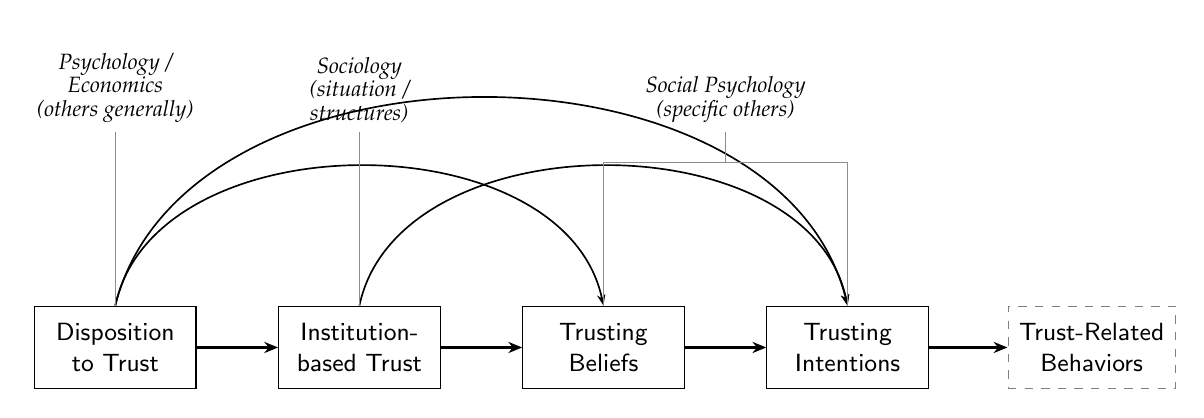
\begin{tikzpicture}[
  box/.style={draw, rectangle, minimum width=2.05cm, minimum height=1.05cm,
              align=center, font=\small\sffamily, inner sep=4pt},
  dbox/.style={draw=black!50, dashed, rectangle, minimum width=2.05cm,
               minimum height=1.05cm, align=center, font=\small\sffamily, inner sep=4pt},
  lbl/.style={font=\footnotesize\itshape, align=center},
  thk/.style={-{Stealth[length=5pt,width=4pt]}, line width=1.4pt},
  thn/.style={-{Stealth[length=4pt,width=3pt]}, line width=0.6pt},
  sub/.style={thin, black!45},
]
%% ---- Boxes (y=0) ----
\node[box]  (D)  at ( 0.0, 0) {Disposition\\to Trust};
\node[box]  (I)  at ( 3.1, 0) {Institution-\\based Trust};
\node[box]  (B)  at ( 6.2, 0) {Trusting\\Beliefs};
\node[box]  (TI) at ( 9.3, 0) {Trusting\\Intentions};
\node[dbox] (TR) at (12.4, 0) {Trust-Related\\Behaviors};

%% ---- Primary thick arrows ----
\draw[thk] (D.east)  -- (I.west);
\draw[thk] (I.east)  -- (B.west);
\draw[thk] (B.east)  -- (TI.west);
\draw[thk] (TI.east) -- (TR.west);

%% ---- Thin skip arrows (arc above boxes) ----
\draw[thn] (D.north)  to[out=78, in=102] (B.north);   %% D -> B
\draw[thn] (D.north)  to[out=76, in=104] (TI.north);  %% D -> TI
\draw[thn] (I.north)  to[out=78, in=102] (TI.north);  %% I -> TI

%% ---- Discipline labels ----
%% Psychology / Economics above D
\node[lbl, above=2.2cm of D] (lD)
  {\textit{Psychology /}\\[-1pt]\textit{Economics}\\[-1pt]\textit{(others generally)}};
\draw[sub] (lD.south) -- (D.north);

%% Sociology above I
\node[lbl, above=2.2cm of I] (lI)
  {\textit{Sociology}\\[-1pt]\textit{(situation /}\\[-1pt]\textit{structures)}};
\draw[sub] (lI.south) -- (I.north);

%% Social Psychology spanning B and TI (bracket)
\node[lbl] at (7.75, 3.15) (lSP)
  {\textit{Social Psychology}\\[-1pt]\textit{(specific others)}};
%% Bracket: stem → horizontal bar → drops to B.north and TI.north
\coordinate (stem) at (7.75, 2.35);
\draw[sub] (lSP.south) -- (stem);
\draw[sub] (6.2, 2.35) -- (9.3, 2.35);
\draw[sub] (6.2, 2.35) -- (B.north);
\draw[sub] (9.3, 2.35) -- (TI.north);
\end{tikzpicture}
\caption{Interdisciplinary model of trust constructs (adapted from McKnight \& Chervany, 2001, Figure~1). Thicker arrows are primary causal paths. Thinner arrows are weaker or mediated links. The dotted box lies outside the formal trust typology.}
\label{fig:mcknight_causal}
\end{figure}

The ``grammar'' of trust (Figure~2 in the original paper) makes the differentiating logic explicit: the trustor is the subject, trust is the verb, and the \textit{direct object} determines the type of trust construct involved.

\begin{center}
\begin{tabular}{llll}
\toprule
\textbf{Subject (Trustor)} & \textbf{Verb} & \textbf{Object (Trustee)} & \textbf{Type} \\
\midrule
The e-commerce consumer & trusts & \textit{the E-vendor} & Interpersonal \\
The e-commerce consumer & trusts & \textit{the web itself} & Institutional \\
The e-commerce consumer & trusts & \textit{others generally} & Dispositional \\
\bottomrule
\multicolumn{4}{l}{\small Adapted from McKnight \& Chervany (2001), Figure 2.}
\end{tabular}
\end{center}

\textbf{Contextual orientation of constructs.} The four constructs differ along two contextual dimensions: whether they are situation-specific or cross-situational, and whether they are person-specific or cross-personal. It makes explicit why collapsing trust into a single score is analytically unsound: each construct has a different contextual scope, and an intervention that affects one need not affect another.

\begin{center}
\begin{tabular}{lcccc}
\toprule
 & \multicolumn{2}{c}{\textbf{Situational}} & \multicolumn{2}{c}{\textbf{Personal}} \\
\cmidrule(lr){2-3}\cmidrule(lr){4-5}
\textbf{Trust Type} & Situation-specific & Cross-situational & Person-specific & Cross-personal \\
\midrule
Disposition to Trust & & \checkmark & & \checkmark \\
Institution-based Trust & \checkmark & & & \checkmark \\
Trusting Beliefs & & \checkmark & \checkmark & \\
Trusting Intentions & & \checkmark & \checkmark & \\
\bottomrule
\multicolumn{5}{l}{\small Adapted from McKnight \& Chervany (2001), Table 3.}
\end{tabular}
\end{center}

\textbf{Methodology.} The paper is a purely conceptual synthesis. It contains no empirical study, no experiment, and no participant data. Its contribution is the taxonomic framework itself: the definitions, the hierarchy of constructs and subconstructs, and the proposed causal model. The authors report that 93 student raters validated the categorisation of trust characteristics, with 71 percent agreement with the authors' assignments. The authors also note that scales for each subconstruct were developed and tested separately, with results to be reported elsewhere.

\textbf{Limitations acknowledged by the authors.} Two limitations are identified. First, crossing disciplinary lines risks losing nuance from original domain-specific definitions; the authors address this by grounding each subconstruct carefully in its originating literature. Second, some subconstructs may not be empirically discriminant in all conditions: particularly benevolence and integrity tend to factor together when the trustor knows little about the trustee. The dispositional and institution-based subconstructs are described as consistently distinguishable.

\textbf{Relevance to this thesis.} The McKnight and Chervany typology provides the theoretical foundation for the three-part trust battery used in this study (Parts E, F, and G of the questionnaire). The three Trusting Beliefs subconstructs retained here --- competence, benevolence, and integrity --- correspond directly to their framework, as adopted by Canales et al.\ (2024) for the avatar trust context. Predictability is not measured as a separate subscale in this study because, as McKnight and Chervany themselves note, it tends to merge with competence and integrity when the trustor and trustee are unfamiliar, which is the case for all participants in a first-impression video study.

The scenario design maps the three constructs onto distinct advisor interactions. Scenario 1 (Career Choice) targets \textit{competence}: the participant must judge whether the advisor has the knowledge and judgment to navigate a complex career trade-off. Scenario 2 (Travel Route) targets \textit{benevolence} alongside competence: the advisor must demonstrate that they are looking out for the participant's specific interests, not giving generic advice. Scenario 3 (Learning Resource) targets \textit{integrity}: the advisor is honest about a trade-off that could undermine their recommendation (the free option has equivalent content), demonstrating transparent reasoning over self-serving simplification.

\textbf{Why Disposition to Trust and Institution-based Trust are not measured.} The remaining two constructs in the McKnight and Chervany typology are excluded from this study for principled reasons that follow directly from the model. Disposition to Trust is a stable personality trait: it is cross-situational and cross-personal, meaning it captures how much a given participant tends to trust people in general, regardless of who they are or what context they appear in. It does not vary based on which avatar a participant just watched. Measuring it three times across three video blocks would yield the same score each time; it cannot function as a within-subjects dependent variable. In a more comprehensive study design it would enter as a between-subjects covariate, measured once per participant. Institution-based Trust is similarly invariant across conditions because every participant in this study encounters the same institutional context, that is, the same survey platform, the same study framing, and the same university ethics-approved environment. None of this changes between C1, C2, and C3. Moreover, the research question is not about the trustworthiness of the study environment but about the trustworthiness of a specific advisor as perceived through their visual rendering. That is precisely the interpersonal domain. Both excluded constructs are antecedents in the McKnight and Chervany causal model: they feed into Trusting Beliefs rather than being outcomes of them. Measuring Trusting Beliefs is therefore the theoretically correct choice for a study whose independent variable is the appearance of a specific other party.

\vspace{8pt}
\subsection{Mayer, Davis \& Schoorman (1995) --- Integrative Model of Trust}

\begin{refbox}
\textbf{Full reference:} Mayer, R. C., Davis, J. H., \& Schoorman, F. D. (1995). An integrative model of organizational trust. \textit{Academy of Management Review}, 20(3), 709--734.\\[4pt]
\textbf{DOI:} \texttt{10.5465/amr.1995.9508080335}
\end{refbox}

\textbf{Core argument.} Prior trust research suffered from conceptual fragmentation: disciplines used definitions that were not interchangeable, making findings hard to compare. Mayer et al.\ synthesised these into one integrative model. Trust is defined as \textit{``the willingness of a party to be vulnerable to the actions of another party based on the expectation that the other will perform a particular action important to the trustor, irrespective of the ability to monitor or control that other party''} (p.~712). Three elements are essential: (1) willingness to be vulnerable; (2) the absence of monitoring and control; (3) a positive expectation about the other party's behaviour. Trust is therefore a disposition toward risk, not a response to certainty.

\textbf{The three trustworthiness factors --- the ABI model.} Trust in a specific other party arises from that party's perceived trustworthiness, decomposed into three independent factors:

\begin{itemize}[leftmargin=2em]
  \item \textbf{Ability:} A cluster of skills and competencies that enable a party to have influence within a specific domain. Ability is domain-specific: a trustee may be highly competent in one area and not in another. In an advisory context, ability concerns whether the advisor has the knowledge and judgment to provide useful guidance on the particular topic at hand.
  \item \textbf{Benevolence:} The extent to which the trustee is believed to want to do good for the trustor, apart from any self-interested motive. Benevolence is relational and specific to the trustor-trustee dyad --- it is not a general trait of kindness but a belief that this trustee specifically cares about this trustor's wellbeing. An advisor with high benevolence would not exploit an informational asymmetry to push the trustor toward an option that serves the advisor's own interests.
  \item \textbf{Integrity:} The trustor's perception that the trustee adheres to a set of principles the trustor finds acceptable. This includes honesty, consistency between stated values and observed actions, and credibility in communication. A trustee with high integrity discloses trade-offs honestly even when doing so is complicated for the trustor to hear.
\end{itemize}

The three factors are conceptually independent and can take different values for the same trustee: a party can be highly able but low in benevolence (competent but self-serving), or high in benevolence but low in ability (caring but ineffective). Collapsing them into a single trust score obscures these distinctions and masks differential effects.

\textbf{Full causal model.} Perceived trustworthiness (ability + benevolence + integrity) produces trust (willingness to be vulnerable), which produces risk-taking behaviour in the relationship. This behavioural outcome --- acting on advice, following a recommendation, selecting a trustee for a consequential task --- sits outside the definition of trust itself but is its downstream consequence. Two moderators are included: (1) the trustor's \textit{propensity to trust}, a stable individual trait that determines how much weight is placed on perceived trustworthiness before much evidence has accumulated; and (2) the \textit{perceived risk} of the situation, which moderates whether trust translates into actual risk-taking behaviour at all.

\textbf{What trust is not.} The authors explicitly distinguish trust from cooperation (which can occur under monitoring), from confidence (which implies certainty, not vulnerability), and from predictability (one can predict an untrustworthy person's behaviour without trusting them). A scale that asks whether participants can predict a trustee's behaviour is not measuring trust.

\textbf{Relevance to this study.} The Mayer et al.\ ABI model is the theoretical foundation for the trust battery in Parts E, F, and G of the questionnaire, as adopted by Canales et al.\ (2024) for the avatar trust context. The three subscales correspond directly: ability (Part E: competence and relevant knowledge), benevolence (Part F: caring and acting in the participant's interest), and integrity (Part G: honesty and transparent reasoning). The forced-choice advisor selection (Part P1) operationalises the risk-taking behavioural outcome that Mayer et al.\ place downstream of trust in their model. Including both the self-report battery and the behavioural measure allows this study to test whether the self-report and behavioural layers dissociate across rendering conditions.

\vspace{8pt}
\subsection{Bartneck et al.\ (2009) --- Godspeed Questionnaire Series}

\begin{refbox}
\textbf{Full reference:} Bartneck, C., Kuli\'{c}, D., Croft, E., \& Zoghbi, S. (2009). Measurement instruments for the anthropomorphism, animacy, likeability, perceived intelligence, and perceived safety of robots. \textit{International Journal of Social Robotics}, 1(1), 71--81.\\[4pt]
\textbf{DOI:} \texttt{10.1007/s12369-008-0001-3}
\end{refbox}

\textbf{Background and motivation.} Robot developers in HRI had been creating their own ad hoc questionnaires without validation, making results from different studies impossible to compare. Bartneck et al.\ conducted a literature review of existing instruments for five key perceptual concepts, then standardised and validated them into a single coherent battery, which they named \textit{Godspeed}. All five subscales use \textbf{5-point semantic differential} format: participants rate their impression of the robot by choosing between two opposing adjective anchors (e.g., $\mathit{Fake} \leftrightarrow \mathit{Natural}$). This format was chosen over Likert items to reduce acquiescence bias and to maintain consistency across subscales. Validation used a within-subjects study with three robot appearance conditions (human, android, masked android); Cronbach's $\alpha$ was computed per condition, with 0.7 as the minimum acceptable threshold following Nunnally (1978).

\textbf{The five Godspeed subscales.}

\medskip
\noindent\textbf{Godspeed I --- Anthropomorphism} \hfill \textit{5 items}

Captures the degree to which participants attribute human form, characteristics, or behavior to the observed entity. Connected directly to the uncanny valley: a robot that scores high on anthropomorphism but fails to match the expectations that score creates will trigger stronger eeriness responses.

\begin{center}
\begin{tabular}{rll}
\toprule
\textbf{Negative anchor} & \textbf{Scale} & \textbf{Positive anchor} \\
\midrule
Fake & 1\;2\;3\;4\;5 & Natural \\
Machinelike & 1\;2\;3\;4\;5 & Humanlike \\
Unconscious & 1\;2\;3\;4\;5 & Conscious \\
Artificial & 1\;2\;3\;4\;5 & Lifelike \\
Moving rigidly & 1\;2\;3\;4\;5 & Moving elegantly \\
\bottomrule
\end{tabular}
\end{center}

Cronbach's $\alpha$: 0.878 (Study 1); 0.929 (human condition), 0.923 (android), 0.856 (masked android) in the within-subjects study. All above threshold.

\medskip
\noindent\textbf{Godspeed II --- Animacy} \hfill \textit{6 items}

Captures perceived aliveness and responsiveness. Grounded in the Piagetian framework: things that move of their own accord, react to stimuli, and interact with their environment are perceived as animate.

\begin{center}
\begin{tabular}{rll}
\toprule
\textbf{Negative anchor} & \textbf{Scale} & \textbf{Positive anchor} \\
\midrule
Dead & 1\;2\;3\;4\;5 & Alive \\
Stagnant & 1\;2\;3\;4\;5 & Lively \\
Mechanical & 1\;2\;3\;4\;5 & Organic \\
Artificial & 1\;2\;3\;4\;5 & Lifelike \\
Inert & 1\;2\;3\;4\;5 & Interactive \\
Apathetic & 1\;2\;3\;4\;5 & Responsive \\
\bottomrule
\end{tabular}
\end{center}

Cronbach's $\alpha$: 0.702 (Study 1); above 0.7 across all conditions in the within-subjects study. The authors note that \textit{Artificial/Lifelike} appears in both Anthropomorphism and Animacy; correlation analysis is recommended when both are used together.

\medskip
\noindent\textbf{Godspeed III --- Likeability} \hfill \textit{5 items}

Captures positive affective appeal and social warmth. Research shows that first impressions form within seconds to minutes: people decide within 30 seconds whether a blind date will succeed, and interviewers know within 1--2 minutes whether a job applicant is a strong candidate. Computers and robots are treated as social actors by the same mechanisms.

\begin{center}
\begin{tabular}{rll}
\toprule
\textbf{Negative anchor} & \textbf{Scale} & \textbf{Positive anchor} \\
\midrule
Dislike & 1\;2\;3\;4\;5 & Like \\
Unfriendly & 1\;2\;3\;4\;5 & Friendly \\
Unkind & 1\;2\;3\;4\;5 & Kind \\
Unpleasant & 1\;2\;3\;4\;5 & Pleasant \\
Awful & 1\;2\;3\;4\;5 & Nice \\
\bottomrule
\end{tabular}
\end{center}

Cronbach's $\alpha$: 0.865 (Study 1); 0.923 (human), 0.878 (android), 0.842 (masked android). All well above threshold.

\medskip
\noindent\textbf{Godspeed IV --- Perceived Intelligence} \hfill \textit{5 items}

Captures the observer's subjective judgment of the entity's intellectual capacity, explicitly distinct from actual computational intelligence. Perceived intelligence depends on behavioral cues: an entity that displays contextually appropriate, non-random behavior is perceived as more intelligent, regardless of whether that behavior is genuinely reasoned or scripted.

\begin{center}
\begin{tabular}{rll}
\toprule
\textbf{Negative anchor} & \textbf{Scale} & \textbf{Positive anchor} \\
\midrule
Incompetent & 1\;2\;3\;4\;5 & Competent \\
Ignorant & 1\;2\;3\;4\;5 & Knowledgeable \\
Irresponsible & 1\;2\;3\;4\;5 & Responsible \\
Unintelligent & 1\;2\;3\;4\;5 & Intelligent \\
Foolish & 1\;2\;3\;4\;5 & Sensible \\
\bottomrule
\end{tabular}
\end{center}

Cronbach's $\alpha$: 0.750, 0.769, 0.763 across three independent studies. All above threshold.

\medskip
\noindent\textbf{Godspeed V --- Perceived Safety} \hfill \textit{3 items}

Captures the observer's subjective sense of comfort and absence of anxiety during interaction. Unlike the four previous subscales, the instruction asks about the participant's own affective state rather than their impression of the robot. Developed by Kulic and Croft from physiological sensor data and validated against heart rate and skin conductance measurements.

\begin{center}
\begin{tabular}{rll}
\toprule
\textbf{Negative anchor} & \textbf{Scale} & \textbf{Positive anchor} \\
\midrule
Anxious & 1\;2\;3\;4\;5 & Relaxed \\
Agitated & 1\;2\;3\;4\;5 & Calm \\
Quiescent & 1\;2\;3\;4\;5 & Surprised \\
\bottomrule
\end{tabular}
\end{center}

Cronbach's $\alpha$: 0.91 in the validation study. Strong correlation with physiological arousal measures established concurrent validity.

\textbf{Which Godspeed subscales are used in this study and which are not.}

\textit{Used:}
\begin{itemize}[leftmargin=2em]
  \item \textbf{Godspeed I (Anthropomorphism) $\to$ Part D of the questionnaire.} This subscale operationalises perceived human-likeness, which is the perceptual axis along which the three conditions differ. C1 (real person) is expected to score highest; C3 (NPR avatar) is expected to score lower than C2 (realistic avatar) because NPR rendering removes photorealistic texture detail and softens skin gradients. Including anthropomorphism ratings allows testing whether differences in eeriness across conditions are mediated by shifts in perceived human-likeness (H5), or whether eeriness changes independently of humanness scores.
  \item \textbf{Godspeed III (Likeability) $\to$ Part C of the questionnaire.} This subscale is the primary affective indicator in this study. Likeability captures warmth, social appeal, and positive first impressions: the affective dimension most directly disrupted by eeriness. If NPR abstraction successfully reduces the uncanny valley response, one mechanism by which it does so is by making the avatar more likeable. Likeability also partially predicts trust: an advisor who is perceived as warm and pleasant is more likely to be listened to and followed. Separating likeability from the trust subscales (Parts E--G) allows the analysis to distinguish affective response from cognitive trust assessment.
\end{itemize}

\textit{Not used, and why:}
\begin{itemize}[leftmargin=2em]
  \item \textbf{Godspeed II (Animacy) --- excluded.} Animacy measures perceived aliveness and biological responsiveness. In this study, all three conditions use the same video recordings with the same movement quality per scenario block. The animation is held constant across C2 and C3 (the critical comparison pair), and C1 is a real person with naturally organic motion. There is no design manipulation targeting animacy perception, so including it would add items without contributing to the core hypotheses. Animacy also overlaps substantially with anthropomorphism at the item level (\textit{Artificial/Lifelike} appears in both), which would require additional factor analysis to disentangle.
  \item \textbf{Godspeed IV (Perceived Intelligence) --- excluded.} Perceived intelligence is covered with greater specificity by the McKnight and Chervany trust subscales in Parts E--G. The Competence trust items (Part E: \textit{This advisor seems knowledgeable about this topic}, \textit{This advisor gave me relevant advice}) are a direct and theory-grounded measure of the same construct as Godspeed IV, but framed in terms of the advisory relationship rather than as a general impression of cognitive ability. Adding Godspeed IV alongside the trust battery would create redundancy and lengthen the questionnaire without adding explanatory power.
  \item \textbf{Godspeed V (Perceived Safety) --- excluded.} Perceived safety measures anxiety and discomfort during physical proximity to a robot. This construct has no meaningful referent in a video-only study where the avatar is not physically co-present and poses no motion hazard. The original scale was validated specifically for industrial robot motion scenarios where the robot's speed and trajectory could create genuine physical threat. Applying it to a seated video advisor would produce floor-effect ratings without variance, making the scale analytically useless in this context.
\end{itemize}

\textbf{General limitation noted by the authors.} Results from Godspeed subscales should be interpreted as comparative tools, not absolute values. Ground truth for constructs like anthropomorphism or likeability is inaccessible: cultural background, prior experience with robots, and individual personality all influence ratings. The questionnaires provide a snapshot that allows conditions to be compared within a study, but absolute scores should not be generalised across different participant populations or stimulus types.

\vspace{8pt}
\subsection{Canales, Roble \& Neff (2024) --- Trust and Avatar Stylisation}

\begin{refbox}
\textbf{Full reference:} Canales, R., Roble, D., \& Neff, M. (2024). The impact of avatar stylization on trust. In \textit{2024 IEEE Conference on Virtual Reality and 3D User Interfaces (VR)}, 418--428.\\[4pt]
\textbf{DOI:} \texttt{10.1109/VR58804.2024.00063}
\end{refbox}

\textbf{Study design.} 66 participants in VR each interviewed three virtual doctors in a 3 (identity) $\times$ 3 (stylisation level) within-subjects design. Three doctor identities (Asian female AF, South Asian male AM, Caucasian male CM) were each rendered at three stylisation levels: photorealistic (Real), semi-realistic (Mid), and caricatured. All responses were pre-recorded using high-quality offline motion capture (Vicon for body, Faceware for face) and played back in Unreal Engine 5 on a Meta Quest 2. The scenario was high-stakes medical: participants imagined they had been diagnosed with a potentially cancerous kidney lump and needed a second opinion. Each doctor answered three preset questions, one designed to address each trust component from the Mayer et al.\ (1995) ABI model.

\textbf{Questionnaire and behavioural measure.} After each doctor interview, participants completed a trust survey on 7-point Likert scales. The survey covered the three Mayer et al.\ trust components:

\begin{itemize}[leftmargin=2em]
  \item \textbf{Ability} --- two items assessing perceived competence and relevant skills
  \item \textbf{Benevolence} --- two items assessing perceived care and alignment with patient interests
  \item \textbf{Integrity} --- two items assessing honesty and adherence to acceptable principles
  \item \textbf{Composite trust} --- one overall trust item
\end{itemize}

All items were 7-point Likert scales. Scale labels were withheld from participants to avoid priming. Dialogues were pre-tested on Mechanical Turk to be statistically equivalent in believability across all three doctor identities. After all three interviews, participants chose their most preferred doctor for a follow-up second opinion and their least preferred --- the primary behavioural trust indicator.

\textbf{Key results.} Style had no significant main effect on any self-report trust dimension (ability: $p = .12$; benevolence partial: $p = .034$; integrity: $p = .16$; composite trust: $p = .13$). Realistic avatars were not trusted more than stylised ones. However, stylisation significantly affected \textit{behavioural} doctor selection ($p = .044$): Mid-style was chosen as most preferred doctor by 48\% of participants, compared to approximately 26\% each for Real and Caricature. The strongest effect was \textit{identity}: CM was consistently rated lower on all trust dimensions and selected as least preferred most often, driven by motion and body language artifacts from the retargeting pipeline rather than visual style.

\textbf{Relevance to this study.} This is the closest prior work to the current study. Three design decisions are adopted directly: (1) the video-based advisor paradigm with pre-recorded scripted responses; (2) the Mayer et al.\ ABI trust battery on 7-point Likert scales (Parts E, F, G of the questionnaire); (3) the forced-choice advisor selection as a behavioural trust indicator (Part P1). The finding that self-reported trust was equivalent across stylisation levels is the empirical basis for H2. The dissociation between self-report (no style effect) and behavioural selection (Mid preferred) is the reason this study includes both measures: a self-report battery alone would have missed the style preference entirely.

\vspace{8pt}
\subsection{Alipour, Hartmann \& Alimardani (2025) --- Systematic Review}

\begin{refbox}
\textbf{Full reference:} Alipour, A., Hartmann, T., \& Alimardani, M. (2025). Would you rely on an eerie agent? A systematic review of the impact of the Uncanny Valley Effect on trust in human-agent interaction. \textit{arXiv preprint arXiv:2505.05543}.\\[4pt]
\textbf{DOI\,/\,arXiv:} \texttt{arXiv:2505.05543} \quad \url{https://arxiv.org/abs/2505.05543}
\end{refbox}

\textbf{Core question.} How does the Uncanny Valley Effect (UVE) impact human trust in agents? This is the first systematic review to map the intersection of UVE research and trust across the empirical literature as a whole.

\textbf{Method.} PRISMA 2020 systematic review. The search covered seven databases (Scopus, Web of Science, PubMed, APA PsycInfo, IEEE Xplore, ProQuest, WorldCat) using the string (\textit{``uncanny valley'' OR ``uncanny effect''}) AND (\textit{trust* OR believab* OR persuas* OR acceptab* OR acceptance OR competen* OR credib*}). The initial pool of 641 records was reduced to 311 after removing duplicates and excluded formats. After two-stage screening (title/abstract then full text), 53 studies were retained. Inter-rater reliability was Fleiss' Kappa $= 0.61$, indicating substantial agreement. Data were extracted using predefined codes covering agent type, modality, study design, UVE measures, trust measures, and key findings.

\textbf{Key observation on interaction type.} 42 out of 53 studies (79\%) used indirect encounters: participants passively viewed static images, videos, or transcripts rather than engaging in live interaction with an agent. Agent types spanned robots ($n = 25$), virtual agents ($n = 21$), chatbots ($n = 2$), and voice-only systems ($n = 2$).

\textbf{Novel trust measurement framework.} The paper's central theoretical contribution is a three-category taxonomy of how trust has been assessed across the literature:

\begin{center}
\begin{tabular}{p{3.5cm}cp{7cm}}
\toprule
\textbf{Category} & \textbf{Studies} & \textbf{What it captures} \\
\midrule
Direct trust measures & 24 & Explicit self-reported trust or trustworthiness ratings \\[4pt]
Trust-related constructs & 11 & Competence, acceptability, credibility, believability, persuasion \\[4pt]
Trust-related intentions & 18 & Behavioural intentions: advice following, willingness to interact, purchase decisions \\
\bottomrule
\end{tabular}
\end{center}

Of the 53 studies, 46 relied exclusively on subjective self-report. Only 7 used objective behavioural measures such as trust games or decision tasks.

\textbf{UVE measurement.} The best-practice measures for capturing the UVE are eeriness ($n = 38$ studies) and creepiness ($n = 4$ studies), which showed the largest effect sizes in the meta-analysis by Diel et al.\ (2021). Broader affective responses such as discomfort, threat, disgust, or anxiety were used in 12 studies. Positive affinity measures (familiarity, likability) appeared in 3 studies.

\textbf{Main findings.} Among the 41 studies that empirically tested the UVE--trust relationship:

\begin{itemize}[leftmargin=2em]
  \item \textbf{17 studies reported a direct effect.} In every case, the direction was the same: UVE diminished trust or trust-related outcomes. The most rigorous example is Mathur and Reichling (2016), who ran a monetary investment game with robot face stimuli and showed that trust followed the same valley-shaped curve as liking: robots falling into the uncanny valley received less money from participants.
  \item \textbf{24 studies (more than half) reported a conditional or indirect effect.} The UVE--trust relationship was moderated or mediated by additional factors. Prominent moderators included: context of use and task type ($n = 6$; e.g., the trust cost of uncanniness was weaker in high-expertise tutoring roles than in low-expertise hotel service roles); age ($n = 3$; Tu et al.\ found that younger and middle-aged adults showed a trust dip for near-human agents while older adults did not); familiarity with the agent ($n = 3$); and personality traits and individual neural differences ($n = 3$).
  \item \textbf{10 studies found no effect.} The UVE was successfully induced but did not translate into reduced trust. Kim (2022) confirmed that hyper-realistic avatars were rated significantly higher on uncanniness and freakiness than cartoonish avatars, yet trustworthiness scores were statistically equivalent across both types.
\end{itemize}

\textbf{Competence as a buffer.} A cross-cutting finding across several no-effect and moderation studies is that perceived competence can counteract the negative influence of eeriness on trust. MacDorman (2019) found that eeriness did not reduce persuasion when the computer-animated agent was perceived as competent. Dai and MacDorman (2018, 2021) reported that warmth and competence predicted advice adherence independently of the agent's realism level. Patel and MacDorman (2015) found that advice quality exerted a stronger influence on compliance than the agent's appearance or rated trustworthiness.

\textbf{Three categories of moderating factors.} The review synthesises all moderation findings into three groups:

\begin{itemize}[leftmargin=2em]
  \item \textbf{User-related:} age, personality traits, individual neural response differences, initial impressions, familiarity and satisfaction with the agent, disconfirmed expectations, perceived identity threat, user self-justification, prior interpersonal trust levels.
  \item \textbf{Agent-related:} design mismatches (e.g., realistic visual appearance with artificial voice), competence, warmth, autonomy, emotional expressiveness, curated imperfections, overall trustworthiness signal.
  \item \textbf{Environment-related:} context of use, task type (social vs.\ mechanical vs.\ empathy-requiring), interaction frequency and repetition.
\end{itemize}

\textbf{Limitations of the existing literature (Table 4 of the paper).}

\begin{center}
\begin{tabular}{p{2.2cm}p{7cm}c}
\toprule
\textbf{Validity} & \textbf{Issue} & \textbf{Studies} \\
\midrule
External & Indirect encounters only; no live interaction & 41 \\
External & No sample size justification via power analysis & 46 \\
External & Narrow or specialist sample & 7 \\
Internal & Limited range of stimuli (often only 2 levels) & 19 \\
Internal & Uncontrolled confounding variables & 23 \\
Internal & Failed or weak manipulation checks & 5 \\
Construct & Measurement robustness issues (single-item scales) & 20 \\
Construct & Sole reliance on subjective self-report & 46 \\
\bottomrule
\end{tabular}
\end{center}

\textbf{Recommendations for future research (Table 5 of the paper).}

\begin{enumerate}[leftmargin=2.5em]
  \item Move toward dynamic, real-time interaction paradigms; add longitudinal designs to track trust formation across multiple sessions.
  \item Combine self-report surveys with objective behavioural measures: trust games, forced-choice tasks, physiological signals (HRV, EEG, pupil size).
  \item Manipulate human-likeness across at least 3--5 levels to reveal the non-linear UVE pattern; measure both eeriness and positive responses (familiarity, likability).
  \item Justify sample sizes through power analysis; ensure diversity across gender, age, and cultural background.
  \item Model the relationship structurally: treat UVE as predictor and trust as outcome, with candidate mediators including emotional discomfort, perceived competence, warmth, anthropomorphism, and threat perception.
\end{enumerate}

\textbf{Relevance to this study.}

\begin{itemize}[leftmargin=2em]
  \item \textbf{Validates the video-based design:} 42 out of 53 reviewed studies used indirect exposure. Video stimuli sit squarely within the established empirical norm and are explicitly classified as an appropriate stimulus type by the authors.
  \item \textbf{Validates combining self-report with a behavioural indicator:} the paper explicitly identifies reliance on self-report alone as a major limitation and recommends pairing surveys with behavioural measures. Part P1 (forced-choice advisor selection) implements exactly this recommendation.
  \item \textbf{Validates eeriness as the primary UVE instrument (Part B):} eeriness is identified as the best-practice measure with the largest effect sizes across the prior meta-analysis (Diel et al., 2021), used in 38 of the 53 reviewed studies.
  \item \textbf{Validates the dual positive/negative measurement approach (Parts B and C):} the paper recommends measuring both negative (eeriness) and positive (likeability, familiarity) dimensions; this is implemented via the Ho and MacDorman eeriness subscale (Part B) and the Godspeed Likeability subscale (Part C).
  \item \textbf{Grounds hypothesis H4} (eeriness negatively predicts trust across conditions): the majority of direct-effect studies confirm this direction, supporting H4 as a correlational prediction.
  \item \textbf{Explains the plausibility of H2} (no significant trust difference between C2 and C3): the 10 no-effect studies and the competence-as-buffer literature both support the expectation that equivalent advice quality can produce equivalent trust across rendering styles, even where eeriness differs.
\end{itemize}

\vspace{8pt}
\subsection{Nowak \& Biocca (2003) --- Agency, Anthropomorphism, and Social Presence}

\begin{refbox}
\textbf{Full reference:} Nowak, K. L. \& Biocca, F. (2003). The effect of the agency and anthropomorphism on users' sense of telepresence, copresence, and social presence in virtual environments. \textit{Presence: Teleoperators and Virtual Environments}, 12(5), 481--494.\\[4pt]
\textbf{DOI:} \texttt{10.1162/105474603322761289}
\end{refbox}

\textbf{Key distinctions.} The paper operationalises three presence dimensions as independent dependent variables. \textit{Telepresence} is the sense of being in the virtual environment itself. \textit{Copresence} is the sense of sharing that space with a specific other person (assessed from both the participant's own perspective and as an attributed property of the partner). \textit{Social presence} is a medium-level property: the perceived capability of the communication channel to convey social cues, irrespective of the specific partner.

\textbf{Study design.} A 2$\times$3 between-subjects experiment with 134 undergraduates. The two independent variables were: (1) \textit{agency} --- whether the interaction partner was described as a human-controlled avatar or a computer-controlled agent; and (2) \textit{visual anthropomorphism} --- high-anthropomorphic (a detailed 3D human face), low-anthropomorphic (a simplified cartoon face with exaggerated eyes), or no image (text-only interaction). Participants spent 15 minutes in a virtual meeting room with the confederate partner, ostensibly preparing for a scavenger hunt.

\textbf{Scales.} Telepresence: 8 items, $\alpha = .88$. Perceived other copresence: 15 items, $\alpha = .90$. Self-reported copresence: 11 items, $\alpha = .78$. Social presence: 9 items on sliding scales.

\textbf{Results.}
\begin{itemize}[leftmargin=2em]
  \item \textbf{Agency had no significant effect} on any presence measure (telepresence, copresence, or social presence). Whether participants believed their partner was human or a bot did not change how connected or present they felt. This challenges the assumption that knowing an agent is human is a prerequisite for meaningful social engagement.
  \item \textbf{Presence of any virtual image} (vs.\ no image) marginally increased telepresence ($p = .12$). Having a visual representation of a partner, even a minimal one, helps participants feel situated in the virtual space.
  \item \textbf{Counterintuitive finding:} low-anthropomorphic images produced significantly \textit{more} copresence ($F = 6.52$, $p = .01$) and social presence ($F = 4.90$, $p = .03$) than high-anthropomorphic images or no image. The high-anthropomorphic condition produced the \textit{least} copresence among the image conditions.
\end{itemize}

\textbf{Explanation offered.} High-anthropomorphic visual representations establish expectations of rich, human-level social responsiveness. When those expectations are not met by the limited behaviour of the scripted virtual confederate, participants experience a gap between expectation and reality, which reduces their sense of connection. Low-anthropomorphic representations do not trigger such high expectations, so the same limited interaction produces a satisfying social experience. This expectation-mismatch mechanism is closely related to the uncanny valley: a highly realistic avatar that fails to meet human-level behavioural expectations is penalised more severely than a less realistic one.

\textbf{Relevance to this thesis.} Nowak and Biocca's counterintuitive finding --- that lower anthropomorphism can produce higher social presence --- provides theoretical support for the prediction that NPR stylisation (C3) need not reduce trust or social engagement relative to the photorealistic avatar (C2). If the realistic C2 avatar establishes higher perceptual expectations that the recorded video cannot fully satisfy, the stylised C3 may perform comparably or better. The paper also operationalises copresence and social presence in ways relevant to interpreting trust ratings across conditions.

\vspace{8pt}
\subsection{Nowak \& Rauh (2005) --- Avatar Appearance and Online Social Perceptions}

\begin{refbox}
\textbf{Full reference:} Nowak, K. L. \& Rauh, C. (2005). The influence of the avatar on online perceptions of anthropomorphism, androgyny, credibility, homophily, and attraction. \textit{Journal of Computer-Mediated Communication}, 11(1).\\[4pt]
\textbf{DOI:} \texttt{10.1111/j.1083-6101.2005.tb00291.x}
\end{refbox}

\textbf{Research question.} How do avatar appearance choices affect how an online interaction partner is perceived in terms of anthropomorphism, credibility, homophily (perceived similarity), and social attraction?

\textbf{Method.} Participants ($n = 177$) were shown 30 different avatar images that varied systematically in human likeness (from abstract geometric icons to photorealistic faces) and gender cues (masculine, feminine, androgynous). Images were presented as representations of potential online interaction partners. Participants completed multi-item validated scales for each dependent variable.

\textbf{Key findings.}
\begin{itemize}[leftmargin=2em]
  \item Avatar human-likeness significantly predicted anthropomorphism ratings: more human-like avatars were perceived as having more human-like thoughts and motivations.
  \item The relationship between human-likeness and credibility was not linear. Highly anthropomorphic but androgynous avatars received the most favourable credibility, homophily, and attraction ratings.
  \item Androgynous avatars (those without strong gender cues) received higher credibility ratings than strongly gendered avatars, suggesting that demographic ambiguity reduces the opportunity for stereotype-based discounting of the partner's credibility.
  \item Participants showed greater social attraction to avatars perceived as most similar to themselves (homophily effect), with similarity assessed both in gender terms and in perceived humanness.
  \item More abstract avatars did not automatically produce lower social perceptions: the relationship depended on the specific perceptual dimension, confirming that avatar appearance effects are multidimensional and not reducible to a simple ``more human-like is better'' principle.
\end{itemize}

\textbf{Relevance to this thesis.} Nowak and Rauh establish that avatar appearance choices reliably affect how an online partner is socially perceived across dimensions closely related to trust: credibility, attraction, and perceived similarity. The finding that social perception is sensitive to anthropomorphism level in a nonlinear way supports the expectation that NPR stylisation will affect perceived credibility of the advisory avatar, while not necessarily in a straightforwardly negative direction.

\vspace{8pt}
\subsection{Weidner et al.\ (2023) --- Systematic Review of Avatars in AR and VR}

\begin{refbox}
\textbf{Full reference:} Weidner, F., Boettcher, G., Arevalo Arboleda, S., Diao, C., Sinani, L., Kunert, C., Gerhardt, C., Broll, W., \& Raake, A. (2023). A systematic review on the visualization of avatars and agents in AR \& VR displayed using head-mounted displays. \textit{IEEE Transactions on Visualization and Computer Graphics}, 29.\\[4pt]
\textbf{DOI:} \texttt{10.1109/TVCG.2023.3247072}
\end{refbox}

\textbf{Scope.} PRISMA systematic review of 72 empirical papers published between 2015 and 2022, studying avatars or agents rendered in AR or VR using HMDs. Sources: ACM Digital Library, IEEE Xplore, SpringerLink, Frontiers, and MIT Press. Inclusion criteria required: HMD use during the study, at least two conditions comparing different avatar visualisation choices, and empirical human participant data. 233 papers screened; 72 included.

\textbf{Rendering style taxonomy.} The 72 included papers used the following style categories (with overlap): abstract ($n = 21$), stickman ($n = 10$), cartoon ($n = 16$), stylized ($n = 20$), robot ($n = 17$), generic realistic ($n = 56$), personalized realistic ($n = 10$), scanned realistic ($n = 3$), video ($n = 5$), point cloud ($n = 6$), translucent ($n = 2$), and hybrid ($n = 3$). The majority used full-body visualization ($n = 50$, 69.4\%).

\textbf{Task domain taxonomy.} Five task domains: (1) physical activity (walking and non-walking); (2) hand interaction (direct and indirect manipulation); (3) communication (dynamic bidirectional and static unidirectional); (4) game-like scenarios; (5) education and training.

\textbf{Key high-level findings.}
\begin{itemize}[leftmargin=2em]
  \item Full-body visualization consistently outperforms partial-body configurations (head-only, head-and-hands) across nearly all measures: embodiment, task performance, presence, and social presence.
  \item Generic realistic avatars significantly outperform other styles for bidirectional communication tasks. Realistic appearance supports richer nonverbal communication through gaze, facial expression, and gesture fidelity.
  \item For game-like and educational tasks, visual fidelity contributes far less: abstract or cartoon avatars perform comparably to realistic ones in task performance and learning outcomes.
  \item Personalized realistic and scanned realistic avatars tend to produce the strongest effects on embodiment and body ownership, though at higher technical cost.
  \item Facial animation and lip synchronisation are under-studied and under-reported: only 22 papers manipulated or controlled for animation quality, despite its known influence on the uncanny valley.
  \item AR and VR findings transfer reasonably well to each other: 47 papers tested in VR only, 12 in AR only, and 13 in both; the basic style effects were broadly consistent across display type.
\end{itemize}

\textbf{Practical guidelines.} The review synthesises seven practitioner guidelines: (1) use generic realistic full-body as a default for communication-oriented applications; (2) give users agency over visible body parts; (3) prioritise realistic styles where interpersonal trust, presence, or social norm adherence matter; (4) for engaging game content or easy training tasks, realistic rendering is not essential; (5) realistic hands improve hand interaction performance; (6) limit visual complexity in learning contexts to avoid distraction; (7) personalized realistic and video avatars can outperform generic realistic when individual identity matters.

\textbf{Relevance to this thesis.} This review provides the widest-scope summary of how rendering style affects avatar-mediated behaviour in immersive environments. Its finding that rendering style significantly affects social perception and communication behaviour across dozens of independent studies corroborates the central motivation for this thesis's user study: that NPR stylisation is a meaningful independent variable with measurable perceptual effects. The review also confirms that avatar visualization research has focused primarily on first-person self-avatars and physical interaction tasks; the present study extends this to third-person advisory contexts and trust formation from scripted video stimuli, filling a gap Weidner et al.\ identify as understudied.

\vspace{8pt}
\subsection{Kuffner dos Anjos \& Pereira (2024) --- Realism and Self-Embodied Avatars}

\begin{refbox}
\textbf{Full reference:} Kuffner dos Anjos, R. \& Madeiras Pereira, J. (2024). Effects of realism and representation on self-embodied avatars in immersive virtual environments. \textit{arXiv preprint}, arXiv:2405.02672.\\[4pt]
\textbf{Preprint:} \texttt{arXiv:2405.02672}
\end{refbox}

\textbf{Research question.} How do avatar realism level and camera perspective (first-person vs.\ third-person) interact to affect sense of embodiment, task performance, and social presence in VR navigation tasks?

\textbf{Study design.} 24 participants performed four navigation tasks (obstacle avoidance by walking, by jumping, by crouching, and object catching) in a 4m$\times$4m physical room tracked by Kinect depth sensors. Three avatar representations were compared: (1) \textit{Abstract} --- spheres for joints, cylinders for limbs, no texture; (2) \textit{Mesh} --- a realistic 3D humanoid mesh driven by Kinect skeleton tracking; (3) \textit{Point Cloud} --- a real-time depth-sensor reconstruction of the participant's actual body. Each was presented in both first-person perspective (1PP) and third-person perspective (3PP), giving 12 conditions, administered in counterbalanced order via Latin Square.

\textbf{Embodiment questionnaire.} Participants rated four embodiment sub-components after each condition: sense of agency (motor control), body ownership (the virtual body felt like their own), self-location (perceived position matched the avatar), and body control (general coordination sense). All items on a 6-point Likert scale.

\textbf{Key results.}
\begin{itemize}[leftmargin=2em]
  \item \textbf{Perspective outweighs representation.} 1PP produced faster task completion times than 3PP for all three avatar types in most tasks. The clearest effect was on the walking task: 1PP with Mesh was significantly faster than all 3PP conditions ($Z = -3.352$, $p = .001$).
  \item \textbf{Mesh in 1PP showed the strongest embodiment:} agency ($Z = -2.687$, $p = .007$), body ownership ($Z = -2.775$, $p = .006$), and self-location ($Z = -3.574$, $p < .001$) were all significantly higher than Abstract or Point Cloud in 1PP.
  \item \textbf{Mesh in 3PP was the worst performing condition} on the obstacle-crouching task ($Z = -3.254$, $p = .001$). The authors attribute this to the uncanny valley: the realistic appearance sets higher behavioural expectations that the imperfect Kinect animation fails to meet when viewed from outside the body.
  \item \textbf{Abstract in 3PP produced higher body ownership} than Mesh in 3PP, and users showed greater spatial confidence (fewer errors in distance estimation) with the abstract avatar.
  \item \textbf{Point Cloud in 3PP showed the highest agency score} ($Z = -2.812$, $p < .01$) but caused visual occlusion problems and occasional rendering artefacts.
\end{itemize}

\textbf{Design guidelines.}
\begin{itemize}[leftmargin=2em]
  \item Avoid mesh avatars in third-person perspective: the uncanny valley is amplified in 3PP because the user can observe the avatar's full body motion.
  \item Use Abstract or Point Cloud representations for third-person spatial navigation tasks.
  \item 1PP with Mesh is the optimal choice for embodiment-critical applications.
\end{itemize}

\textbf{Relevance to this thesis.} This paper extends uncanny valley research to the self-embodiment domain, demonstrating that imperfect animation on a realistic mesh amplifies negative perception when the avatar is observed from outside the body. This is directly analogous to why the photorealistic C2 advisory avatar, observed by participants as a video, may produce higher eeriness than the stylised C3: subtle imperfections in facial animation or expression timing are perceptually more costly against a photorealistic appearance than against a stylised one.

\vspace{8pt}
\subsection{Alimardani, de Roode, Vaitonyt\.{e} \& Louwerse (2024) --- Appearance, Voice, and Trust in Virtual Agent Collaboration}

\begin{refbox}
\textbf{Full reference:} Alimardani, M., de Roode, R., Vaitonyt\.{e}, J., \& Louwerse, M. M. (2024). Effect of a virtual agent's appearance and voice on uncanny valley and trust in human-agent collaboration. In \textit{Proceedings of the 24th ACM International Conference on Intelligent Virtual Agents (IVA '24)}, Article 5. ACM.\\[4pt]
\textbf{DOI:} \texttt{10.1145/3652988.3673970}
\end{refbox}

\textbf{Research question.} Does a mismatch between a virtual agent's visual appearance (humanlike vs.\ robotic) and voice (humanlike vs.\ synthesised robotic) affect uncanny valley perception, anthropomorphism attribution, and trusting behaviour in a collaborative task?

\textbf{Study design.} A $2\times2$ between-subjects factorial experiment. Independent variables: (1) \textit{agent appearance} --- humanlike (photorealistic 3D virtual human face) or robotic (clearly mechanical robot face); (2) \textit{agent voice} --- humanlike (natural sounding synthesis) or robotic (clearly synthetic speech). Four resulting conditions: Humanlike/Humanlike (matched), Humanlike/Robotic (mismatch), Robotic/Humanlike (mismatch), Robotic/Robotic (matched). $n = 80$ participants (20 per condition) performed an emotion recognition task in which the virtual agent presented images and offered recommendations. After each trial the participant could accept or override the agent's recommendation, so trusting behaviour was operationalised as the proportion of agent recommendations adopted across trials.

\textbf{Dependent measures.} Anthropomorphism (Godspeed Anthropomorphism subscale), uncanny valley perception (6-item eeriness scale from Ho \& MacDorman, 2010), and trusting behaviour (advice-following rate).

\textbf{Key results.}
\begin{itemize}[leftmargin=2em]
  \item \textbf{Anthropomorphism:} A significant appearance $\times$ voice interaction. The mismatch Robotic/Humanlike condition elevated anthropomorphism ratings above the matched Robotic/Robotic condition --- the human voice ``upgraded'' perceived humanness beyond what the robotic appearance alone suggested.
  \item \textbf{Eeriness:} The Humanlike/Robotic mismatch (realistic face + robotic voice) produced the highest eeriness ratings, significantly above all matched conditions. Mismatching modalities amplified the uncanny valley response.
  \item \textbf{Trusting behaviour:} \textbf{No significant main or interaction effect} of appearance or voice on advice-following rate. All four conditions produced statistically equivalent trust behaviour. This is the critical null result.
\end{itemize}

\textbf{Interpretation.} A clean dissociation: manipulating the agent's appearance and voice changes anthropomorphism and eeriness perception, but does not change whether participants follow its advice. The authors interpret this through the Mayer et al.\ (1995) ABI lens: when the agent's demonstrated competence (consistent and reliable recommendations) is held constant, perceptual shifts in appearance do not alter the trust placed in that competence.

\textbf{Relevance to this thesis.} This paper provides the strongest single-study support for H2 (NPR stylisation does not significantly reduce trust). The design isolates visual appearance while holding task competence constant, which mirrors the C2 vs.\ C3 comparison where both conditions deliver identical scripted advice. If even a dramatic mismatch combining a humanlike face with a robotic voice does not reduce trusting behaviour, a shift from photorealistic to NPR-stylised rendering of the same advisor is similarly unlikely to produce a significant trust reduction.

\vspace{8pt}
\subsection{Dubosc, Gorisse, Lefrou, Richir \& Christmann (2025) --- Avatar Stylisation and Facial Expression Intensity}

\begin{refbox}
\textbf{Full reference:} Dubosc, C., Gorisse, G., Lefrou, T., Richir, S., \& Christmann, O. (2025). Effect of avatar stylization and facial expression intensity in virtual interactions. \textit{Virtual Reality}, Springer Nature. Published online 8 October 2025.\\[4pt]
\textbf{DOI:} \texttt{10.1007/s10055-025-01238-6}
\end{refbox}

\textbf{Research question.} Does the avatar's stylisation level affect co-presence, eeriness, and trustworthiness in a virtual face-to-face interaction? Does the intensity of facial expressions modulate these effects?

\textbf{Study design.} 40 participants in a VR face-to-face interaction. A professional actress performed scripted dialogue; her motion-capture performance was retargeted simultaneously onto three avatar versions: \textit{stylised} (cartoon-like, simplified geometry, high colour saturation), \textit{semi-realistic} (intermediate stylisation, visible skin texture), and \textit{realistic} (photorealistic, subsurface scattering, full texture detail). Three expression intensity levels were applied: \textit{reduced} (movements dampened to 50\%), \textit{unaltered} (original), and \textit{augmented} (amplified to 150\%). Stylisation was the within-subjects factor; expression intensity was between-subjects. Mixed $3 \times 3$ design.

\begin{figure}[htbp]
\centering
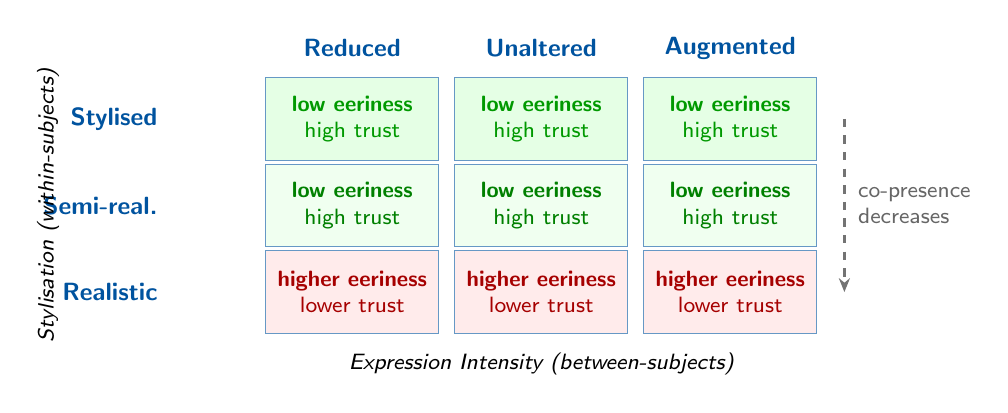
\begin{tikzpicture}[
  cell/.style={draw=konstanzblue!60, fill=#1, rectangle,
               minimum width=2.2cm, minimum height=1.05cm,
               align=center, font=\footnotesize\sffamily, inner sep=3pt},
  hdr/.style={font=\small\sffamily\bfseries\color{konstanzblue}, align=center},
]
%% Column headers (Expression Intensity)
\node[hdr] at (2.3, 3.6) {Reduced};
\node[hdr] at (4.7, 3.6) {Unaltered};
\node[hdr] at (7.1, 3.6) {Augmented};

%% Row headers (Stylisation)
\node[hdr, rotate=0, anchor=east] at (-0.05, 2.7) {Stylised};
\node[hdr, rotate=0, anchor=east] at (-0.05, 1.6) {Semi-real.};
\node[hdr, rotate=0, anchor=east] at (-0.05, 0.5) {Realistic};

%% Axis labels
\node[font=\footnotesize\sffamily\itshape, anchor=north] at (4.7, -0.15)
  {Expression Intensity (between-subjects)};
\node[font=\footnotesize\sffamily\itshape, rotate=90, anchor=south] at (-1.3, 1.6)
  {Stylisation (within-subjects)};

%% Stylised row -- low eeriness, high trust across all expression levels
\foreach \x in {2.3, 4.7, 7.1} {
  \node[cell=green!10!white] at (\x, 2.7)
    {\color{green!60!black}\textbf{low eeriness}\\\color{green!60!black}high trust};
}
%% Semi-realistic row -- also low eeriness
\foreach \x in {2.3, 4.7, 7.1} {
  \node[cell=green!6!white] at (\x, 1.6)
    {\color{green!50!black}\textbf{low eeriness}\\\color{green!50!black}high trust};
}
%% Realistic row -- higher eeriness
\foreach \x in {2.3, 4.7, 7.1} {
  \node[cell=red!8!white] at (\x, 0.5)
    {\color{red!65!black}\textbf{higher eeriness}\\\color{red!65!black}lower trust};
}

%% Co-presence annotation
\draw[-{Stealth[length=5pt,width=4pt]}, thick, black!55, dashed]
  (8.55, 2.7) -- (8.55, 0.5);
\node[right, font=\footnotesize\sffamily, align=left, text=black!60] at (8.6, 1.6)
  {co-presence\\decreases};
\end{tikzpicture}
\caption{Experimental design of Dubosc et al.\ (2025). Stylisation is the within-subjects factor (rows); expression intensity is between-subjects (columns). The main effect of stylisation on eeriness and trustworthiness was significant across all expression intensity conditions. No interaction was found.}
\label{fig:dubosc_design}
\end{figure}

\textbf{Outcome measures.} Co-presence (7-point scale adapted from Nowak \& Biocca, 2003), eeriness (adapted from Ho \& MacDorman, 2010), and trustworthiness (5-point rating).

\textbf{Key results.}
\begin{itemize}[leftmargin=2em]
  \item \textbf{Co-presence:} Significant main effect of stylisation ($F = 7.83$, $p < .001$, $\eta^2_p = .18$). Stylised produced significantly greater co-presence than realistic ($p = .002$). No effect of expression intensity. No interaction.
  \item \textbf{Eeriness:} Significant main effect of stylisation ($F = 11.24$, $p < .001$, $\eta^2_p = .23$). Stylised and semi-realistic produced significantly lower eeriness than realistic ($p < .001$ and $p = .004$ respectively). No significant difference between stylised and semi-realistic. No expression intensity effect. No interaction.
  \item \textbf{Trustworthiness:} Significant main effect of stylisation ($F = 6.94$, $p < .001$, $\eta^2_p = .16$). Stylised and semi-realistic were rated significantly \textit{more} trustworthy than realistic ($p = .001$ and $p = .009$ respectively). No interaction.
\end{itemize}

\textbf{Interpretation.} The photorealistic avatar triggers a subtle uncanny valley response even among participants who do not consciously label it as eerie, and this reduces social confidence in it. Stylised avatars sitting clearly outside the uncanny zone do not trigger this response and are consequently rated as more socially reliable. The absence of any interaction between stylisation and expression intensity confirms that the expression content of scripted content does not confound the stylisation effect.

\textbf{Relevance to this thesis.} This is the most directly relevant new paper to the current study. Both the C2 vs.\ C3 comparison and the Dubosc et al.\ realistic vs.\ stylised comparison manipulate rendering style while holding performance content constant. The finding that stylised avatars produce lower eeriness \textit{and} higher trustworthiness than photorealistic avatars is strong prior evidence that H1 will be supported (C3 lower eeriness than C2) and that H2 may in fact yield null or even a positive direction. The no-interaction result further validates the assumption that holding the adviser script constant across conditions is sufficient to isolate the rendering effect.

\vspace{8pt}
\subsection{Tao, Liu, Qiu \& Li (2025) --- Network Meta-Analysis of Avatar Realism and Perceptual Experience}

\begin{refbox}
\textbf{Full reference:} Tao, Z., Liu, Y., Qiu, J., \& Li, S. (2025). Impact of virtual avatar appearance realism on perceptual interaction experience: a network meta-analysis. \textit{Frontiers in Psychology}, 16, Article 1624975. Published 3 December 2025.\\[4pt]
\textbf{DOI:} \texttt{10.3389/fpsyg.2025.1624975}
\end{refbox}

\textbf{Research question.} What is the quantitative effect of virtual avatar appearance realism on three perceptual outcomes --- attractiveness, trustworthiness, and eeriness --- as synthesised across the empirical literature?

\textbf{Method.} Network meta-analysis (NMA). A standard meta-analysis pools studies comparing the same two conditions. NMA extends this using indirect comparisons: if Study A compares Low vs.\ Medium and Study B compares Medium vs.\ High, NMA can estimate the Low vs.\ High effect without a study that directly compares them, enabling simultaneous ranking across all levels. Search period: April 2015 to April 2025, four databases. Inclusion: studies that manipulated avatar appearance realism as an independent variable and measured at least one target outcome. \textbf{13 studies with 2,343 participants included.} Realism was coded into three levels: \textit{low} (abstract, cartoon, stylised), \textit{medium} (semi-realistic, realistic-but-not-photorealistic), and \textit{high} (photorealistic, scanned).

\medskip
\noindent\textbf{Key findings at a glance.}

\begin{center}
\begin{tabular}{lccc}
\toprule
\textbf{Outcome} & \textbf{Low realism} & \textbf{Medium realism} & \textbf{High realism} \\
\midrule
Attractiveness & lowest & middle & \textbf{highest} \\
Trustworthiness & lowest & middle & \textbf{highest} \\
Eeriness & low & \textbf{peak (valley!)} & medium \\
\bottomrule
\multicolumn{4}{l}{\small Bold indicates the extreme value on that dimension.}
\end{tabular}
\end{center}

\begin{itemize}[leftmargin=2em]
  \item \textbf{Attractiveness:} High realism significantly more attractive than both medium and low (SUCRA: High = 83\%, Medium = 46\%, Low = 21\%). Linear increase with realism.
  \item \textbf{Trustworthiness:} High realism significantly more trustworthy than both medium and low (SUCRA: High = 79\%, Medium = 44\%, Low = 27\%). Medium and low not significantly different from each other.
  \item \textbf{Eeriness:} Medium realism produced the strongest eeriness, significantly higher than both high and low (SUCRA for high eeriness: Medium = 82\%, Low = 19\%, High = 49\%). This is the quantitative confirmation of the uncanny valley: semi-realistic avatars are the most eerie, while both abstract and photorealistic avatars are less eerie.
\end{itemize}

\textbf{Interpretation.} The first NMA-level quantitative confirmation that the uncanny valley is specific to medium realism levels, not an artefact of individual study design. High-realism avatars achieve the second peak (lower eeriness than medium, highest attractiveness and trustworthiness). Low-realism avatars avoid the valley by remaining far from the ambiguous near-human zone.

\textbf{Relevance to this thesis.} The C2 avatar (Avaturn photorealistic) sits near the high-realism zone; the C3 avatar (NPR-stylised) moves toward the low-realism zone. The NMA predicts that this shift reduces eeriness because both high and low realism score lower than medium. However, the NMA also shows that trustworthiness follows realism monotonically: low-realism avatars score the lowest on trustworthiness. This provides the countervailing pressure motivating H2: the two hypotheses together test whether the eeriness reduction from C2 to C3 can be achieved without a significant trustworthiness cost that the meta-analysis would predict.

\vspace{8pt}
\subsection{Cihodaru-\c{S}tefanache \& Podina (2025) --- Uncanny Valley in Embodied Conversational Agents}

\begin{refbox}
\textbf{Full reference:} Cihodaru-\c{S}tefanache, \c{S}. \& Podina, I. R. (2025). The uncanny valley effect in embodied conversational agents: a critical systematic review of attractiveness, anthropomorphism, and uncanniness. \textit{Frontiers in Psychology}, 16, Article 1625984.\\[4pt]
\textbf{DOI:} \texttt{10.3389/fpsyg.2025.1625984}
\end{refbox}

\textbf{Scope.} PRISMA 2020 systematic review investigating how ECA (embodied conversational agent) design features and user characteristics interact to produce uncanny valley responses, with three target outcomes: attractiveness, anthropomorphism, and uncanniness. ECAs are defined as screen-based or VR virtual humans capable of dialogue and non-verbal communication.

\textbf{Method.} Search across ACM Digital Library, IEEE Xplore, Scopus, ProQuest, and Web of Science. Initial pool: 21,897 records. After deduplication, title/abstract screening, and full-text review: \textbf{29 studies included.} Methodological quality was assessed using a standardised checklist; most included studies were rated as weak to moderate quality.

\textbf{ECA design factors identified as uncanny valley predictors.}
\begin{itemize}[leftmargin=2em]
  \item \textbf{Physical appearance:} skin texture realism, hair rendering quality, eye contact behaviour, and blink rate were the most commonly studied features. All showed significant effects on uncanniness when manipulated.
  \item \textbf{Non-verbal communication:} gesture fluency, lip synchronisation accuracy, and facial expression timing all affected the UVE. Asynchronies between speech and lip movement, or between emotional content and expression onset, consistently amplified eeriness.
  \item \textbf{Voice-appearance consistency:} the most consistent cross-study finding. Mismatches between visual appearance realism and voice quality amplify the UVE. An ECA with a highly realistic face paired with a synthetic voice, or vice versa, received higher uncanniness ratings than matched agents.
  \item \textbf{Stylisation:} studies comparing stylised versus realistic ECAs consistently found that stylised agents produced lower uncanniness scores. Deliberate low-realism stylisation is the most frequently recommended avoidance strategy.
\end{itemize}

\textbf{User characteristics identified as moderators.}
\begin{itemize}[leftmargin=2em]
  \item Age: younger adults showed more pronounced UVE responses than older adults.
  \item Technology familiarity: more experience with virtual agents attenuated UVE responses.
  \item Individual disgust sensitivity predicted eeriness ratings independently of stimulus properties.
\end{itemize}

\textbf{Checklist for Avoiding the UVE in ECAs} (three-domain practical output of the review):
\begin{enumerate}[leftmargin=2.5em]
  \item \textit{Physical appearance:} use consistent realism across all visual features; avoid partial stylisation (e.g.\ realistic eyes with cartoon hair); consider deliberate low-realism stylisation when uncanny valley avoidance is prioritised over visual fidelity.
  \item \textit{Non-verbal communication:} ensure accurate lip synchronisation; match facial expression timing and intensity to speech prosody; maintain a natural blink rate (average 15--20 blinks per minute).
  \item \textit{Multimodal consistency:} match visual realism level to voice quality; avoid appearance-voice modality mismatches.
\end{enumerate}

\textbf{Relevance to this thesis.} The recommendation to use consistent stylisation across all visual features validates the approach of applying a single NPR shader uniformly to the Avaturn avatar (C3) rather than selectively stylising only certain body regions. The voice-appearance consistency finding is also relevant to interpreting C2 vs.\ C3 differences: both conditions use the same recorded voice, meaning C2 (realistic appearance + human voice) is fully consistent while C3 (stylised appearance + human voice) introduces a moderate mismatch. This mismatch could amplify eeriness for C3 relative to what pure appearance-level stylisation would produce, which should be acknowledged as a limitation in the discussion of H1.

\newpage
%% ============================================================
\section{NPR --- Nonphotorealistic Rendering}
%% ============================================================

\subsection{Gooch et al.\ (1998) --- A Nonphotorealistic Lighting Model for Technical Illustration}

\begin{refbox}
\textbf{Full reference:} Gooch, A., Gooch, B., Shirley, P., \& Cohen, E. (1998). A non-photorealistic lighting model for automatic technical illustration. In \textit{Proceedings of SIGGRAPH 1998} (pp. 447--452). ACM.\\[4pt]
\textbf{DOI:} \texttt{10.1145/280814.280950}
\end{refbox}

\textbf{Problem.} Standard Phong shading maps surface illumination to a grayscale or colour gradient that fills the entire dynamic range from black (shadow) to white (highlight). Technical illustrators solve a different problem: they need every surface region to be clearly readable, so they confine shading to the midtone range and reserve pure black for outlines and pure white for specular highlights. This produces drawings where form is unambiguous regardless of the lighting angle, which is rarely achievable with Phong shading.

\textbf{The tone-transfer model.} Gooch et al.\ propose a shading function that replaces the Phong diffuse term with a cool-to-warm tone shift:
\[
  I = \frac{1 + \hat{l} \cdot \hat{n}}{2} \cdot k_{\text{warm}} + \frac{1 - \hat{l} \cdot \hat{n}}{2} \cdot k_{\text{cool}}
\]
where $\hat{l}$ is the unit vector toward the light and $\hat{n}$ is the surface normal. The warm colour $k_{\text{warm}} = k_{\text{yellow}} + \beta k_d$ and the cool colour $k_{\text{cool}} = k_{\text{blue}} + \alpha k_d$ blend the object's diffuse colour $k_d$ with yellow and blue tint colours. The parameters $\alpha, \beta \in [0, 1]$ control how much the object's own colour contributes versus the pure tint. This construction keeps all shading values in the midtone range: faces pointing toward the light receive a warm midtone, those pointing away receive a cool midtone, and neither reaches the extremes of black or white. Black is reserved for drawn outlines; white for Phong specular highlights.

\textbf{GPU implementation approximation.} The paper describes a real-time approximation using two Phong lights placed symmetrically about the view direction: one with positive and one with negative intensity, with ambient set to the average of warm and cool. This can be computed without a special shader by exploiting standard Phong lighting parameters. Specular highlights are rendered white and placed as a final compositing step, ensuring the highlight ``pops'' against both warm and cool shaded regions.

\textbf{Metal shading.} For metallic surfaces, the authors propose alternating stripes of varying intensity along the parametric axis of maximum curvature. Stripe intensities are sampled randomly in $[0, 0.5]$ and colours interpolate between the light source colour and the surface reflected direction, approximating the Fresnel-like angular highlight characteristic of polished metal. The result resembles hand-drawn technical metal shading.

\textbf{Key principle.} Gooch cool-to-warm shading makes shape readable by encoding orientation information in hue rather than luminance. A viewer can perceive the 3D form of a shaded Gooch surface even when it is reduced to greyscale, because the hue shift maps onto a consistent orientation cue. This is distinct from toon shading (see Lake et al.\ below), which quantises luminance rather than shifting hue.

\textbf{Relevance to this thesis.} Gooch et al.\ (1998) established the principle that NPR shading can use the full spectral gamut to convey surface orientation without sacrificing readability. The cool-to-warm model is cited in the thesis as the foundation of nonphotorealistic illumination design and motivates the warm/cool split used in early NPR tests before the toon quantisation approach was adopted.

\vspace{8pt}
\subsection{Lake et al.\ (2000) --- Stylized Rendering for Real-Time 3D Animation}

\begin{refbox}
\textbf{Full reference:} Lake, A., Marshall, C., Harris, M., \& Blackstein, M. (2000). Stylized rendering techniques for scalable real-time 3D animation. In \textit{Proceedings of NPAR 2000: First International Symposium on Nonphotorealistic Animation and Rendering} (pp. 13--20). ACM.\\[4pt]
\textbf{DOI:} \texttt{10.1145/340916.340918}
\end{refbox}

\textbf{Context.} This paper describes techniques developed and deployed at Shiny Entertainment for the commercial game \textit{Messiah} (2000). It is notable as one of the first accounts of toon shading implemented in a shipped product, and its techniques became the standard template for real-time NPR in games.

\textbf{Quantised diffuse shading.} The core toon shading technique replaces continuous diffuse lighting with a 1D texture lookup. The Lambertian diffuse factor $\max(\hat{l} \cdot \hat{n}, 0)$ is computed per vertex and used as a texture coordinate into a 1D artist-painted ramp texture. The ramp contains discrete colour bands separated by hard steps. Because the ramp is authored by an artist, the number of bands, the colour of each band, and the sharpness of transitions are fully under artistic control and can be painted per-character or per-material type.

\textbf{Inverted hull (geometry outline).} Object outlines are generated by duplicating the mesh and rendering the duplicate with backface culling inverted (front-facing polygons are culled). The duplicate mesh is inflated along vertex normals by a small offset, so only the silhouette shell is visible around the original mesh. The shell is rendered in a solid dark colour. Because this technique operates in object space, it scales naturally with the character's LOD system: lower-polygon LODs still produce clean outlines without any image-space processing cost.

\textbf{Scalability and LOD integration.} A key design requirement was that the techniques had to work transparently across all LOD levels of the game's characters. The geometry outline passes this requirement because it is a mesh operation; the quantised diffuse ramp passes it because it is a per-vertex computation. The paper documents the performance cost as negligible at the LOD levels used in the game.

\textbf{Artistic authoring.} Because the diffuse ramp is a hand-painted 1D texture, artists retain full control over the visual output. Different characters can have stylistically distinct shading (warmer highlight colours, cooler shadows, different band counts) without changing any rendering code.

\textbf{Relevance to this thesis.} Lake et al.\ (2000) introduced the two foundational real-time NPR techniques used throughout this project: quantised diffuse toon shading (V1 in the Meta Avatar shader pipeline, as well as the Avaturn V1 and Jody V1 shaders) and the inverted hull outline. The geometry outline is directly implemented in \texttt{V1\_ToonShading\_GeometryOutline.shader} across all three avatar pipelines.

\vspace{8pt}
\subsection{Isenberg et al.\ (2003) --- A Developer's Guide to Silhouette Algorithms}

\begin{refbox}
\textbf{Full reference:} Isenberg, T., Freudenberg, B., Halper, N., Schlechtweg, S., \& Strothotte, T. (2003). A developer's guide to silhouette algorithms for polygonal models. \textit{IEEE Computer Graphics and Applications}, 23(4), 28--37.\\[4pt]
\textbf{DOI:} \texttt{10.1109/MCG.2003.1210862}
\end{refbox}

\textbf{Scope.} This survey paper systematically classifies all known approaches to computing and rendering silhouette edges for polygonal 3D meshes. It is aimed at graphics developers who need to choose among the available algorithms for specific real-time or offline NPR applications. The paper covers image space, hybrid, and object space approaches, and provides a practical decision table.

\textbf{Definition of silhouette.} For a polygonal mesh, a silhouette edge is any edge shared by exactly one front-facing and one back-facing polygon with respect to the current camera position. This is the geometric definition: $(\hat{n}_1 \cdot \hat{v} \leq 0) \neq (\hat{n}_2 \cdot \hat{v} \leq 0)$, where $\hat{v}$ is the view direction and $\hat{n}_1$, $\hat{n}_2$ are the face normals of the two adjacent triangles. Smooth-surface silhouettes satisfy $\hat{n} \cdot (\mathbf{x} - \mathbf{C}) = 0$ (the surface normal is perpendicular to the view ray at that point).

\textbf{Image space algorithms.} Use a depth buffer, normal buffer, or colour buffer rendered from the scene; apply a per-pixel edge detection filter (such as Sobel or Roberts Cross on normals or depth). Advantages: fast, handles self-intersecting geometry, independent of polygon count. Limitations: pixel-level precision only, cannot control line width analytically, produces aliased output at edges between objects rather than geometric silhouettes, and cannot distinguish silhouette edges from colour or texture edges.

\textbf{Hybrid algorithms.} Detect silhouette edges in object space (using the geometric criterion above) then render them using image-space techniques (stencil buffer or overdraw). Examples include Raskar and Cohen's backface enlargement and Gooch et al.'s environment-map method. These allow stylised line widths while using hardware rasterisation. Limitations: two render passes required; silhouettes must be computed per frame.

\textbf{Object space algorithms.} Compute silhouette edges directly on the geometry:
\begin{itemize}[leftmargin=2em]
  \item \textit{Trivial algorithm:} iterate all mesh edges and test the face-orientation criterion for each. $O(n)$ per frame; straightforward to implement; slow for dense meshes.
  \item \textit{Precomputation approaches:} project silhouette candidates onto a Gaussian sphere; use hierarchical octrees or dual 4D representations to prune non-silhouette edges rapidly. Suitable for static meshes; fails with full skeleton animation.
  \item \textit{Stochastic (Markosian et al.):} randomly sample a subset $O(\sqrt{n})$ of edges per frame; statistically, only about $\sqrt{n}$ edges are actually silhouette in any frame. Probabilistic but fast; misses isolated silhouette edges occasionally.
\end{itemize}

\textbf{Decision table (Table 1).} The paper provides a table mapping requirements to recommended algorithm class:
\begin{itemize}[leftmargin=2em]
  \item Real-time, arbitrary animated mesh: image space or hybrid.
  \item Guaranteed silhouette completeness: object space trivial or precomputed.
  \item Stroke-level stylisation (variable width, pressure, brush): object space.
  \item Static or slowly animated mesh: precomputed object space.
\end{itemize}

\textbf{Key limitation identified.} Geometry-only silhouette detection captures boundary edges between front- and back-facing polygons, but misses interior crease lines, colour edges, and texture discontinuities. Image space methods recover interior edges but are not true geometric silhouettes.

\textbf{Relevance to this thesis.} Isenberg et al.\ (2003) motivate the progression from V1 (geometry outline) to the image space edge detection in V2 and V3. The geometry outline captures only silhouette edges in object space; interior crease lines and colour boundaries visible in the face and clothing require screen space gradient operators. The paper's limitation note --- that geometry-only edge capture misses these features --- is the direct design motivation for developing V2 (normal edge detection) and V3 (Sobel colour edge detection).

\vspace{8pt}
\subsection{Gonzalez \& Woods (2018) --- Digital Image Processing (4th edition)}

\begin{refbox}
\textbf{Full reference:} Gonzalez, R. C. \& Woods, R. E. (2018). \textit{Digital Image Processing} (4th edition). Pearson/Prentice Hall.\\[4pt]
\textbf{ISBN:} \texttt{978-0133356724}
\end{refbox}

\textbf{Scope.} Standard graduate-level textbook for spatial and frequency domain image processing. The chapters most directly cited in this thesis are Chapter 3 (spatial filtering), Chapter 10 (image segmentation via gradients and edges), and the appendix on colour models.

\textbf{Sobel operator.} Gonzalez and Woods define the Sobel gradient as two $3\times3$ convolution kernels:
\[
  G_x = \begin{pmatrix} -1 & 0 & 1 \\ -2 & 0 & 2 \\ -1 & 0 & 1 \end{pmatrix}, \qquad
  G_y = \begin{pmatrix} -1 & -2 & -1 \\ 0 & 0 & 0 \\ 1 & 2 & 1 \end{pmatrix}
\]
The gradient magnitude is $\|\mathbf{G}\| = \sqrt{G_x^2 + G_y^2}$, approximated in practice as $|G_x| + |G_y|$. The Sobel kernel applies implicit central difference differentiation while simultaneously weighting the centre row/column twice as heavily as the corner rows/columns, giving a small degree of smoothing and improved isotropy compared to simpler gradient operators.

\textbf{Roberts Cross operator.} A $2\times2$ diagonal gradient operator:
\[
  G_1 = \begin{pmatrix} 1 & 0 \\ 0 & -1 \end{pmatrix}, \qquad G_2 = \begin{pmatrix} 0 & 1 \\ -1 & 0 \end{pmatrix}
\]
Roberts Cross responds to diagonal edges and is computationally cheaper than Sobel (4 multiplications vs.\ 8 per output pixel). It is less noise-tolerant but suitable for detecting diagonal surface transitions, which is why it is used alongside the depth normal proxy in the V5 (Hierarchical) shader.

\textbf{Gaussian smoothing.} A discrete approximation to the 2D Gaussian $G(x,y) = e^{-(x^2+y^2)/2\sigma^2}$. Convolved with an image before differentiation, it suppresses high-frequency noise that would otherwise dominate the gradient signal. The standard deviation $\sigma$ controls the scale at which features are detected: large $\sigma$ detects coarse edges and misses fine detail; small $\sigma$ detects fine detail but remains sensitive to noise.

\textbf{BT.601 luminance weights.} For converting RGB colour images to greyscale before edge detection:
\[
  L = 0.299 R + 0.587 G + 0.114 B
\]
These weights reflect the relative sensitivity of the human visual system to each colour channel and are defined in the ITU-R BT.601 broadcast standard. Using these weights rather than equal-weight averaging produces greyscale images that perceptually match the luminance of the original colour image.

\textbf{Laplacian of Gaussian (LoG).} The second derivative of the Gaussian, $\nabla^2 G(x,y)$, applied as a convolution kernel. Zero crossings of the LoG response mark intensity edges. The textbook derives the discrete LoG approximation kernel and describes the zero-crossing detection procedure.

\textbf{Relevance to this thesis.} Gonzalez and Woods provide the mathematical basis for all edge detection operators used across the NPR pipeline: the Sobel kernels in V3 (Sobel edge detection), the Gaussian pre-smoothing in V4 (Gaussian Sobel), the Roberts Cross in V5 (Hierarchical), and the BT.601 luma weights used throughout for greyscale conversion of RGB colour buffers. The textbook is the authoritative source for the mathematical definitions accompanying these techniques in Chapter 4 of the thesis.

\vspace{8pt}
\subsection{Marr \& Hildreth (1980) --- Theory of Edge Detection}

\begin{refbox}
\textbf{Full reference:} Marr, D. \& Hildreth, E. (1980). Theory of edge detection. \textit{Proceedings of the Royal Society of London B: Biological Sciences}, 207(1167), 187--217.\\[4pt]
\textbf{DOI:} \texttt{10.1098/rspb.1980.0020}
\end{refbox}

\textbf{Theoretical contribution.} Marr and Hildreth proposed the first biologically motivated computational theory of edge detection. Their central claim is that the visual system detects edges not by directly computing intensity gradients, but by first smoothing the image at multiple spatial scales and then locating zero crossings of the Laplacian of the smoothed signal. The smoothing function they identify as biologically appropriate is the Gaussian, because it is the unique linear filter that simultaneously minimises spatial spread (localisation) and frequency spread (noise sensitivity).

\textbf{The Laplacian of Gaussian (LoG) operator.} The proposed operator $\nabla^2(G * I)$ --- the Laplacian of the Gaussian-smoothed image --- produces a response that changes sign at intensity discontinuities in the smoothed image. These zero crossings form closed contours in the image, which Marr and Hildreth identify as the \textit{raw primal sketch}: the first stage of visual representation. Unlike gradient-based operators (Sobel, Roberts), the LoG naturally produces edges that are closed curves, reflecting the topological constraint that physical objects have closed boundaries.

\textbf{Scale-space principle.} The Gaussian smoothing scale $\sigma$ determines the spatial resolution at which zero crossings are computed. Large $\sigma$ values suppress fine detail and noise; small $\sigma$ values preserve fine detail. The paper argues that edge detection should be performed at multiple $\sigma$ scales and the results combined: features that appear consistently across scales are more likely to correspond to real physical boundaries than those that appear only at fine scales.

\textbf{Biological evidence.} Marr and Hildreth review psychophysical evidence (Mach bands, subjective contours, masking experiments) and anatomical evidence (receptive field profiles of retinal ganglion cells and lateral geniculate nucleus neurons) consistent with LoG-like processing in the early visual system. The difference-of-Gaussians (DoG) approximation of the LoG matches the known centre-surround structure of ganglion cell receptive fields.

\textbf{Relevance to this thesis.} Marr and Hildreth establish the theoretical principle that pre-smoothing with a Gaussian before computing intensity derivatives is necessary for robust edge detection, not merely empirically useful. This principle directly motivates the V4 (Gaussian Sobel) shader, in which a Gaussian blur is applied to the colour buffer before the Sobel gradient is computed, reducing the UV seam noise and skin-texture noise that affected V3. The LoG concept also contextualises the Canny detector (below), which extends Marr and Hildreth's ideas with non-maximum suppression and hysteresis thresholding.

\vspace{8pt}
\subsection{Canny (1986) --- A Computational Approach to Edge Detection}

\begin{refbox}
\textbf{Full reference:} Canny, J. (1986). A computational approach to edge detection. \textit{IEEE Transactions on Pattern Analysis and Machine Intelligence}, 8(6), 679--698.\\[4pt]
\textbf{DOI:} \texttt{10.1109/TPAMI.1986.4767851}
\end{refbox}

\textbf{Optimality criteria.} Canny posed edge detection as an optimisation problem with three criteria: (1) \textit{detection} --- the detector should respond to all real edges and not respond to non-edges; (2) \textit{localisation} --- detected edges should be as close as possible to the true edge positions; (3) \textit{single response} --- each real edge should produce exactly one detector response, not multiple. He proved that the optimal filter for these three criteria is well approximated by the first derivative of a Gaussian.

\textbf{The four-stage pipeline.}
\begin{enumerate}[leftmargin=2.5em]
  \item \textbf{Gaussian smoothing.} The input image is convolved with a Gaussian $G_\sigma$ at scale $\sigma$. This suppresses noise that would otherwise dominate the gradient in the next step.
  \item \textbf{Gradient computation.} The gradient magnitude $M = \sqrt{G_x^2 + G_y^2}$ and direction $\theta = \arctan(G_y/G_x)$ are computed using first-derivative kernels.
  \item \textbf{Non-maximum suppression.} Each gradient magnitude pixel is compared to its two neighbours in the direction of the gradient. If the pixel is not a local maximum along this direction, it is suppressed to zero. This thins wide gradient responses to single-pixel-wide ridges.
  \item \textbf{Double-threshold hysteresis.} Two thresholds $T_{\text{high}}$ and $T_{\text{low}}$ are applied. Pixels with $M > T_{\text{high}}$ are strong edges and kept unconditionally. Pixels with $M < T_{\text{low}}$ are rejected. Pixels with $T_{\text{low}} \leq M \leq T_{\text{high}}$ are kept only if they are spatially connected to a strong edge. This reduces isolated noise responses while preserving weak edges that are part of longer contours.
\end{enumerate}

\textbf{Relevance to this thesis.} The Canny detector establishes that Gaussian pre-smoothing is not just practically useful but theoretically optimal before gradient-based edge detection. This motivates V4 (Gaussian Sobel), which applies Gaussian pre-smoothing before the Sobel gradient. The full Canny pipeline is not reproduced in the fragment shader (non-maximum suppression and hysteresis require multi-pass access to neighbouring pixels, which is not available in a single-pass fragment hook), but the first two stages --- Gaussian smoothing and gradient computation --- are directly implemented in V4.

\vspace{8pt}
\subsection{Barla et al.\ (2006) --- X-Toon: An Extended Toon Shader}

\begin{refbox}
\textbf{Full reference:} Barla, P., Thollot, J., \& Markosian, L. (2006). X-Toon: An extended toon shader. In \textit{Proceedings of NPAR 2006: 4th International Symposium on Nonphotorealistic Animation and Rendering} (pp. 127--132). ACM.\\[4pt]
\textbf{DOI:} \texttt{10.1145/1138450.1138471}
\end{refbox}

\textbf{Motivation.} Standard toon shading uses a 1D texture lookup keyed on the Lambertian diffuse factor $\hat{n} \cdot \hat{l}$. This encodes only how strongly the surface is lit, and produces a flat, depth-agnostic style: two faces at different distances from the camera with the same orientation relative to the light receive identical shading. Barla et al.\ extend the toon shader with a second dimension to encode view-dependent information such as depth or surface orientation relative to the viewer.

\textbf{Extension 1 --- Tone Detail (2D texture).} The 1D toon ramp is replaced with a 2D texture indexed by two coordinates: $u = \hat{n} \cdot \hat{l}$ (the standard diffuse tone) and $v = D \in [0,1]$ (the detail level). The $v$ axis can be mapped to any view-dependent scalar:
\begin{itemize}[leftmargin=2em]
  \item \textit{Depth-based}: $D = 1 - \log(z / z_{\min}) / \log(z_{\max} / z_{\min})$ --- objects farther from the camera receive a different row of the 2D texture, enabling aerial perspective and depth-of-field effects within a single toon pass.
  \item \textit{Orientation-based}: $D = |\hat{n} \cdot \hat{v}|^r$ --- surfaces facing the viewer (high $|\hat{n} \cdot \hat{v}|$) receive a different row than surfaces at grazing angles, enabling silhouette darkening or backlighting effects.
\end{itemize}
The 2D texture is painted freely by the artist: the entire visual space of the shader is under artistic control, not constrained to a function of the lighting alone.

\textbf{Extension 2 --- Shape Detail (Normal Field Abstraction).} The vertex normals of the mesh are replaced with a blend between the original normals and the normals of an abstract proxy shape (sphere, cylinder, ellipse, or flat disc). A global blending parameter $\alpha \in [0,1]$ controls the degree of abstraction. At $\alpha = 0$, the original detailed mesh normals are used; at $\alpha = 1$, the surface shades as if it were the proxy shape, flattening interior creases while preserving the overall silhouette. Barla et al.\ term this blended normal field the \textit{Normal Field Abstraction}. The abstraction level can be keyframed or linked to the depth axis $D$, allowing surfaces to abstract as they recede from the viewer.

\textbf{Performance.} Table 1 of the paper measures rendering time on a Pentium 4 + ATI Radeon 9800. X-Toon is approximately 18--21\% slower than standard 1D toon shading across four test models and three screen resolutions. This overhead is acceptable for real-time use.

\textbf{Effects achievable.} Aerial perspective (distant objects stylistically faded), depth-of-field suggestion, near-silhouette glow, backlighting, abstract interior with preserved contour, plastic vs.\ metal distinction via different 2D texture rows.

\textbf{Relevance to this thesis.} X-Toon introduced the concept of a \textit{detail axis} --- a continuous scalar $D$ that parameterises how much surface detail is resolved in the final rendering. This concept directly motivates the Avaturn \texttt{XToon\_2DRamp.shader} and the corresponding Jody XToon shader. The Normal Field Abstraction concept is also central to the thesis argument: it shows that toon shading can deliberately control the level of surface detail visible, making it a principled tool for managing perceived avatar complexity and potentially for navigating the uncanny valley.

\vspace{8pt}
\subsection{Kyprianidis et al.\ (2009) --- Image Abstraction by Anisotropic Kuwahara Filtering}

\begin{refbox}
\textbf{Full reference:} Kyprianidis, J. E., Kang, H., \& D\"{o}llner, J. (2009). Image and video abstraction by anisotropic Kuwahara filtering. \textit{Computer Graphics Forum} (Pacific Graphics), 28(7).\\[4pt]
\textbf{DOI:} \texttt{10.1111/j.1467-8659.2009.01574.x}
\end{refbox}

\textbf{The Kuwahara filter (1976).} The classical Kuwahara filter divides a square neighbourhood around each pixel into four overlapping rectangular sub-regions. It computes the mean and variance of pixel values within each sub-region and assigns the output pixel the mean of the sub-region with the lowest variance. The effect is to smooth uniformly within coherent regions while preserving edges, because the sub-region on the ``less noisy'' side of an edge is selected. The filter was originally designed for medical image denoising but produces a characteristic painterly oil-painting effect. Its main defect is block artefacts caused by the four rectangular sub-regions, and instability at edges where sub-regions span both sides of an intensity boundary.

\textbf{Structure tensor.} Kyprianidis et al.\ compute the local image structure tensor from the spatial derivatives of the image:
\[
  \mathbf{G} = \begin{pmatrix} f_x^2 & f_x f_y \\ f_x f_y & f_y^2 \end{pmatrix}
\]
smoothed by a Gaussian with standard deviation $\sigma_s$. The eigenvalues $\lambda_1 \geq \lambda_2$ of this tensor describe the local gradient distribution. The anisotropy measure $A = (\lambda_1 - \lambda_2)/(\lambda_1 + \lambda_2)$ ranges from 0 (isotropic, uniform region or noise) to 1 (fully anisotropic, strong edge). The dominant eigenvector gives the local orientation $\phi$ of the principal gradient direction.

\textbf{Anisotropic filter shape.} The filter neighbourhood is an ellipse $\Omega = \{\mathbf{x} : \|\mathbf{S}\mathbf{R}_{-\phi}\mathbf{x}\| \leq h\}$, where $\mathbf{R}_{-\phi}$ is a rotation by the local orientation angle and $\mathbf{S} = \text{diag}(\alpha/(\alpha+A),\, (\alpha+A)/\alpha)$ is a scaling matrix that elongates the ellipse along the local edge direction in proportion to the anisotropy $A$. In uniform regions ($A \approx 0$), the ellipse is nearly circular; at strong edges ($A \approx 1$), the ellipse elongates to span the edge rather than crossing it.

\textbf{Weighted sector voting.} The ellipse is divided into $N = 8$ equal sectors. For each sector $i$, the mean $m_i$ and standard deviation $s_i$ of pixel values are computed. The output is the weighted sum:
\[
  \text{output} = \frac{\sum_i \alpha_i m_i}{\sum_i \alpha_i}, \qquad \alpha_i = \frac{1}{(1 + s_i)^q}
\]
where $q = 8$. This assigns higher weight to sectors with lower standard deviation (more uniform), effectively selecting the most coherent side of any edge without producing block artefacts.

\textbf{GPU implementation.} Encoded as four RGBA render texture samples (four sectors per channel, two samples to cover 8 sectors). At $512\times512$ resolution with $\sigma_r = 3.0$, $\sigma_s = 1.0$, $N = 8$, the filter runs at approximately 12fps on a GeForce GTX 280 (2009 hardware). Temporal coherence is excellent without motion estimation because the filter respects local edge orientation, which is geometrically stable under slow animation.

\textbf{Limitation noted.} The structure tensor computation requires access to a smoothed structure tensor image computed from the full frame, which is a separate render pass producing a texture. For the anisotropic version to be implemented, a prior render pass must generate and store the structure tensor map. This is not possible within a single-pass fragment shader hook.

\textbf{Relevance to this thesis.} Kyprianidis et al.\ (2009) provide the theoretical basis for the Kuwahara painterly filter implemented as V6 in the Meta Avatar shader pipeline (\texttt{NPREffect\_Kuwahara2.cginc}) and the corresponding shaders for Avaturn and Jody. The thesis implements the isotropic variant of Kuwahara (classical rectangular sub-regions, not the anisotropic elliptical variant) because the fragment shader hook does not permit the separate structure tensor render pass required by the full anisotropic version. This limitation is explicitly documented: the anisotropic filter would provide better edge-aligned strokes but requires a multi-pass pipeline that exceeds the SDK's single-pass constraint.

\vspace{8pt}
\subsection{Praun et al.\ (2001) --- Real-Time Hatching}

\begin{refbox}
\textbf{Full reference:} Praun, E., Hoppe, H., Webb, M., \& Finkelstein, A. (2001). Real-time hatching. In \textit{Proceedings of SIGGRAPH 2001} (pp. 579--584). ACM.\\[4pt]
\textbf{DOI:} \texttt{10.1145/383259.383295}
\end{refbox}

\textbf{Hatching in NPR.} Hatching is a traditional hand-drawing technique in which groups of parallel strokes convey surface tone, material properties, and 3D form simultaneously through stroke density, direction, and spacing. In darker regions, strokes are denser; on curved surfaces, stroke directions follow principal curvature directions to convey form. Cross-hatching adds perpendicular strokes at even darker tones. The challenge for real-time 3D hatching is maintaining stroke coherence across frames, across different surface parameterisations, and across a continuous range of tones.

\textbf{Tonal Art Maps (TAMs).} The core contribution of the paper is the Tonal Art Map: a 2D grid of mip-mapped images. The grid is indexed by tone $t$ (columns; $t = 0$ is white paper, $t = 5$ is darkest hatching) and mip level $\ell$ (rows; $\ell = 0$ is the finest detail level). Each cell contains a greyscale image of hatch strokes. The defining property is \textit{nesting}: every stroke appearing in cell $(t, \ell)$ also appears in all cells $(t', \ell')$ with $t' \geq t$ and $\ell' \geq \ell$. This means that as the tone becomes darker, strokes are \textit{added} but never moved or removed. As the resolution decreases (higher mip level), strokes are wider but fewer. Nesting ensures that tone transitions and resolution changes never produce popping artefacts: the image changes incrementally.

\textbf{TAM construction.} The paper describes a greedy stroke-placement algorithm that fills each TAM cell iteratively. Starting from the lightest tone, strokes are placed to minimize the error between the current partial TAM and the target tone. At darker tones, additional strokes are placed without moving existing ones (nesting constraint). Cross-hatching strokes are added at tones 4 and 5. The algorithm produces TAMs that closely match artist-drawn hatch styles.

\textbf{Rendering.} At runtime, each triangle face has a single dominant tone assigned via its Lambertian diffuse factor (same as toon shading). Rather than a hard-threshold band, the renderer blends between two adjacent tone columns using the fractional tone value, and interpolates the three vertex tone values using barycentric coordinates. This produces six texture samples per fragment (two adjacent tone columns, blended at each of three triangle vertices) combined in two hardware dot products --- a technique the authors call a ``6-way blend.'' The resulting frame rate is 20--40fps for models of 7,500--15,000 faces on a 933MHz Pentium III with a GeForce2 GPU.

\textbf{Lapped textures.} The paper also addresses the challenge of applying TAMs to arbitrary mesh topology without UV seams. The authors use lapped textures: overlapping, irregularly shaped texture patches that cover the surface with a consistent stroke direction field derived from the principal curvature. The patches overlap at their alpha boundaries, hiding seam lines.

\textbf{Relevance to this thesis.} Praun et al.\ (2001) introduced the TAM paradigm, which establishes that real-time hatching with full tone and resolution continuity is achievable through careful pre-computation of the texture content. This technique is cited in the thesis as the foundational reference for hatching-style NPR, while noting that it is not directly implemented: the implementation constraint of a single fragment pass precludes the multi-texture blending and per-face tone assignment that TAMs require without a geometry pass. The \texttt{HalftoneHatching.shader} in \texttt{Assets/Shaders/CommonNPRShaders/} implements a simplified screen-space hatching effect without full TAM-compliant tone nesting.

\vspace{8pt}
\subsection{Roberts (1963) --- Machine Perception of Three-Dimensional Solids}

\begin{refbox}
\textbf{Full reference:} Roberts, L. G. (1963). \textit{Machine perception of three-dimensional solids} (Ph.D.\ thesis). Massachusetts Institute of Technology, Lincoln Laboratory Report TR-315.\\[4pt]
\textbf{Note:} Doctoral thesis; no DOI. Available via MIT DSpace and ResearchGate (\url{https://www.researchgate.net/publication/220695992}).
\end{refbox}

\textbf{Historical significance.} Roberts' thesis is the founding document of edge detection in computer vision. Written in 1963 before the term ``computer vision'' existed as a discipline, it describes a system that processes a photograph of a polyhedral scene and extracts a three-dimensional geometric description. The thesis introduced the \textit{Roberts Cross operator} --- a pair of $2\times2$ convolution kernels detecting diagonal intensity gradients --- as the first systematic mathematical approach to locating edges in digitised images.

\textbf{The Roberts Cross kernels.} To locate intensity boundaries, Roberts applies discrete gradient approximations along the two diagonal directions:
\[
  G_1 = \begin{pmatrix} 1 & 0 \\ 0 & -1 \end{pmatrix}, \qquad G_2 = \begin{pmatrix} 0 & 1 \\ -1 & 0 \end{pmatrix}
\]
The gradient magnitude at each pixel is estimated as $\|G\| = \sqrt{G_1^2 + G_2^2}$, or approximated for speed as $|G_1| + |G_2|$. The diagonal orientation detects 45$^\circ$ and 135$^\circ$ edge directions.

\textbf{Why $2\times2$ and not $3\times3$.} Roberts chose $2\times2$ kernels due to the computational constraints of 1963 hardware (MIT TX-2 computer) and the mathematical minimum: a $2\times2$ discrete operator is the smallest structure capable of computing a diagonal finite difference. The limitation is that the gradient centre falls between pixel corners, introducing a half-pixel positional offset. Later operators (Sobel 1968, Prewitt 1970) improved noise tolerance using $3\times3$ kernels that incorporate more surrounding context at higher cost.

\textbf{Broader contribution.} Roberts built the first complete pipeline from photograph to 3D model: edge detection on the digitised image, line fitting to edge outputs, 3D geometry extraction assuming polyhedral structure, and hidden-line removal for arbitrary viewpoints. Experimental results on actual photographs of polyhedral objects demonstrated successful 3D reconstruction, making this one of the first demonstrations of automated scene understanding from images.

\textbf{Relevance to this thesis.} The Roberts Cross operator is used in the V5 (Hierarchical) shader as the colour-edge component of the three-cue fusion: the $2\times2$ diagonal kernels are applied to the screen-space colour buffer to detect surface colour transitions not captured by the depth proxy or normal derivatives. Currently cited via Gonzalez \& Woods (2018), which derives the Roberts kernels mathematically. Citing the original thesis correctly attributes the operator to its source and situates it within the historical lineage of edge detection preceding the Sobel, Marr-Hildreth, and Canny approaches also used in V3--V5.

\vspace{8pt}
\subsection{Kumar \& Poornima (2019) --- Comprehensive Survey on Nonphotorealistic Rendering}

\begin{refbox}
\textbf{Full reference:} Kumar, T. \& Poornima, B. G. (2019). A comprehensive survey on non-photorealistic rendering and benchmark developments for image abstraction and stylization. \textit{Iran Journal of Computer Science}, Springer Nature.\\[4pt]
\textbf{DOI:} \texttt{10.1007/s42044-019-00034-1}
\end{refbox}

\textbf{Scope.} Structured review of NPR techniques from 1963 to approximately 2017. Organises the entire field into five technique families and proposes a benchmark evaluation framework. It is the most cited recent NPR survey addressing both 2D and 3D stylisation methods within a single taxonomy.

\textbf{Taxonomy of NPR techniques.}

\begin{center}
\begin{tabular}{p{3.0cm}p{8.5cm}}
\toprule
\textbf{Category} & \textbf{Description and representative methods} \\
\midrule
Stroke-based rendering & Simulates individual artistic strokes (hatching, watercolour, oil paint). Includes Tonal Art Maps (Praun et al., 2001) and brush stroke simulation. \\[4pt]
Colour image analogy & Transfers the style of an exemplar image onto a target using texture transfer. Includes Hertzmann et al.'s (2001) image analogies. \\[4pt]
Region-based rendering & Segments the image into coherent regions and applies flat or gradated colouring. Includes cel shading and Voronoi mosaic effects. \\[4pt]
Image filtering abstraction & Applies local image filters to reduce detail while preserving large-scale structure. Includes Kuwahara filtering (Kyprianidis et al., 2009), bilateral filtering, and mean-shift segmentation. \\[4pt]
Stylisation & Direct transformation of shading, colour mapping, and tone, typically real-time. Includes toon shading (Lake et al., 2000), X-Toon (Barla et al., 2006), and Gooch lighting (Gooch et al., 1998). \\
\bottomrule
\end{tabular}
\end{center}

\textbf{Benchmark evaluation criteria.} Visual consistency (coherence across frames), preservation of structural features (edges and shapes remain readable), artistic fidelity (match to target style), and computational cost (real-time capability). These four criteria map directly onto the evaluation framework for the NPR techniques in this thesis.

\textbf{Historical trajectory.} From stroke-based offline rendering systems of the 1990s (hours per frame) to image-space and stylisation techniques of the 2000s (real-time capable) to data-driven and neural approaches of the 2010s.

\textbf{Relevance to this thesis.} Kumar and Poornima's taxonomy provides a single citable survey for placing the eight NPR techniques implemented in this project within the broader literature. V1 (toon shading, V2 X-Toon, inverted hull outline) falls in \textit{stylisation}. V3 (Sobel), V4 (Gaussian Sobel), and V5 (Hierarchical) fall in \textit{image filtering abstraction}. V6--V8 (Kuwahara variants) are image filtering abstraction with painterly qualities overlapping \textit{stroke-based rendering}. The paper can be cited in Chapter 2 (Related Work) to orient the reader before the technique-by-technique discussion.

\vspace{8pt}
\subsection{Wisessing, Dingliana \& McDonnell (2016) --- Perception of Lighting and Shading for Animated Virtual Characters}

\begin{refbox}
\textbf{Full reference:} Wisessing, P., Dingliana, J., \& McDonnell, R. (2016). Perception of lighting and shading for animated virtual characters. In \textit{Proceedings of the ACM Symposium on Applied Perception (SAP 2016)}.\\[4pt]
\textbf{DOI:} \texttt{10.1145/2931002.2931015}
\end{refbox}

\textbf{Research question.} How does shading style (CG-shaded vs.\ toon-shaded) and lighting configuration interact to affect the perceived emotional intensity and appeal of animated virtual characters?

\textbf{Stimulus design.} A professional animator keyframed ten dramatic emotional sentences using a virtual character, each conveying a specific emotion (anger, fear, sadness, surprise, happiness, disgust). Each sentence was rendered in two shading styles (CG with subsurface scattering vs.\ toon flat colour bands with outline), four lighting directions (above, front-below, side, rear), and three lighting intensities (low, medium, high contrast key-to-fill ratio). Participants ($n = 36$) rated each stimulus on: emotion recognition accuracy (which emotion?), emotional intensity (how strongly expressed?), and character appeal.

\textbf{Key results.}
\begin{itemize}[leftmargin=2em]
  \item \textbf{Shading style significantly affected emotional intensity:} CG-shaded renders were rated as conveying significantly more intense emotions than toon-shaded renders of the same performance ($p < .001$). The magnitude was approximately 0.8--1.2 points on a 7-point scale across emotions.
  \item \textbf{Emotion recognition accuracy was not significantly affected by shading style:} participants identified the correct emotion at similar rates regardless of shading. Intensity of the perceived emotion changed; what emotion was perceived did not.
  \item \textbf{Lighting direction had little effect} on perceived emotional intensity. Below-lighting reduced appeal ($p = .02$).
  \item \textbf{High-contrast lighting reduced appeal:} high key-to-fill ratio (deep shadows) was rated less appealing than medium and low contrast ($p < .05$).
\end{itemize}

\textbf{Interpretation.} Toon shading softens the emotional signal of the animation. Photorealistic rendering amplifies subtle facial cues (micro-expressions, shadow detail in wrinkles and skin creases) that toon shading flattens away. Recognition accuracy being preserved means toon-shaded avatars remain comprehensible as social actors while reducing the perceptual ``loudness'' of their facial signals.

\textbf{Relevance to this thesis.} This paper provides a psychophysical explanation for why NPR stylisation may reduce eeriness. If toon shading softens subtle emotional cues in the animation, it simultaneously softens the cues that produce uncanny valley responses (slightly wrong expression timing, subtly unnatural skin movement) and the cues that make the avatar feel intensely realistic. The finding that \textit{recognition accuracy} is preserved while \textit{intensity} is reduced is directly relevant to H1: a toon-shaded avatar may produce lower eeriness without losing communicative clarity.

\vspace{8pt}
\subsection{Wisessing, Zibrek, Cunningham, Dingliana \& McDonnell (2020) --- Enlighten Me: Brightness and Shadow for Character Emotion and Appeal}

\begin{refbox}
\textbf{Full reference:} Wisessing, P., Zibrek, K., Cunningham, D. W., Dingliana, J., \& McDonnell, R. (2020). Enlighten Me: Importance of brightness and shadow for character emotion and appeal. \textit{ACM Transactions on Graphics}, 39(3), Article 30.\\[4pt]
\textbf{DOI:} \texttt{10.1145/3383195}
\end{refbox}

\textbf{Background.} Following the 2016 SAP finding that shading style affects emotional intensity, this paper investigates within each shading style how the specific parameters of lighting --- brightness and shadow depth --- affect character appeal and eeriness. The question is whether the same effects observed across shading styles can be reproduced within a single style by varying lighting parameters.

\textbf{Study design.} Three experiments; primary results from Experiment 3. A $2$ (shading style: CG vs.\ toon) $\times$ 4 (key light brightness levels) $\times$ 4 (key-to-fill ratio levels) within-subjects design, $n = 36$ participants. Characters expressed three emotions (neutral, happy, sad). Participants rated character appeal (1--7) and eeriness (1--7).

\textbf{Key results.}
\begin{itemize}[leftmargin=2em]
  \item \textbf{Increasing key light brightness significantly increased appeal} ($F = 14.3$, $p < .001$, $\eta^2 = .19$) and significantly \textit{decreased eeriness} ($F = 9.7$, $p < .001$, $\eta^2 = .13$) for both shading styles.
  \item \textbf{Reducing the key-to-fill ratio (lighter shadows) significantly increased appeal} ($F = 11.2$, $p < .001$, $\eta^2 = .15$) and significantly \textit{decreased eeriness} ($F = 8.1$, $p < .001$, $\eta^2 = .12$).
  \item \textbf{Eeriness reduction was larger for CG rendering than for toon.} CG characters were more eerie at baseline and benefited more from brighter, lighter-shadow lighting. Toon characters were already less eerie and showed a smaller absolute change.
  \item \textbf{Psychophysical model:} appeal varies as a function of key-to-fill ratio $r$ following a power law: $\text{appeal} = a \cdot r^{-b}$, providing a quantitative prediction of optimal lighting parameters.
\end{itemize}

\textbf{Interpretation.} Eeriness is not solely a property of avatar geometric or textural realism: it is also modulated by the tonal distribution of the shading. Bright, evenly-lit characters with shallow shadows are consistently rated as less eerie and more appealing across both rendering styles. Toon shading's structural properties (lighter mid-tones, painted flat bands without deep luminance-range shadows) align with the low-eeriness lighting configuration.

\textbf{Relevance to this thesis.} Toon shading by definition produces lighter shadow regions than CG rendering: the shadow bands are painted to a constant colour rather than following the full dynamic range of a Lambertian model. This structural property directly maps onto Wisessing et al.'s finding that lighter shadows reduce eeriness. The V1 toon shading in this project uses a warm light band and a cool mid-shadow band without deep black shadows, which matches the low-eeriness lighting configuration identified here. This paper supplies a psychophysical mechanism for why the NPR avatar (C3) may produce lower eeriness than the photorealistic avatar (C2): even if the NPR stylisation did not move the avatar out of the uncanny zone, the inherent tonal flatness of toon shading would still reduce eeriness through the brightness-shadow mechanism documented here.

\vspace{8pt}
\subsection{Petikam, Anjyo \& Rhee (2021) --- Shading Rig: Art-Directable Stylised Shading for 3D Characters}

\begin{refbox}
\textbf{Full reference:} Petikam, L., Anjyo, K., \& Rhee, T. (2021). Shading Rig: Dynamic art-directable stylised shading for 3D characters. \textit{ACM Transactions on Graphics}, 40(5), Article 205.\\[4pt]
\textbf{DOI:} \texttt{10.1145/3461696}
\end{refbox}

\textbf{Problem.} Standard real-time toon shading (Lake et al., 2000) places the light-to-shadow boundary at a threshold derived from the Lambertian dot product $\hat{l} \cdot \hat{n}$. As the character moves or the lighting direction changes, this boundary slides across the surface, producing visually unstable shading that animators working in hand-drawn cel animation styles specifically try to avoid. Professional animated productions (such as \textit{Spider-Man: Into the Spider-Verse}) require artists to manually reshape shadow boundaries per frame to maintain a consistent visual look independent of physically computed lighting. This is not feasible at real-time frame rates.

\textbf{The shading rig concept.} Inspired by facial rigging in character animation, Petikam et al.\ propose the shading rig: a parameterised collection of artist-defined edits to the toon shading output that can be interpolated and blended at runtime.

\begin{itemize}[leftmargin=2em]
  \item Artists define a set of \textit{shading states}: different poses of the light/shadow boundary across the character surface, painted using a direct manipulation tool.
  \item Each state is associated with a control parameter (light direction angle or scene lighting condition).
  \item At runtime the system interpolates between states using a learned interpolation function (a small neural network, approximately 100 parameters).
  \item The result is toon shading that respects artistic intent as lighting changes, rather than mechanically following the Lambertian threshold.
\end{itemize}

\textbf{Implementation.} A Unity shader with a pre-computation pipeline for baking the shading state space from artist-painted examples. The mesh UV coordinates store shading state offsets. Runtime cost of the interpolation network is negligible.

\textbf{Evaluation.} User study ($n = 26$) comparing shading rig output to standard toon shading across animations with varying lighting. Shading rig received significantly higher ratings on visual consistency and artistic fidelity ($p < .001$).

\textbf{Relevance to this thesis.} The shading rig represents the current state of the art in production toon shading for 3D characters. The V1 implementation in this project uses a fixed threshold approach (Lake et al., 2000) because the SDK integration constraint limits the NPR implementation to a single fragment shader hook without the pre-computed state-space baking or the multi-state mesh UV parameterisation that the shading rig requires. Petikam et al.\ contextualise this limitation: the shading rig would produce superior artistic output but is architecturally incompatible with the Meta Avatars SDK's material management system. Citing this paper allows the thesis to acknowledge the gap between the V1 implementation and the production solution without being obligated to close it.

\vspace{8pt}
\subsection{Riefard et al.\ (2024) --- Player Preferences for NPR Artistic Styles in 3D Game Characters}

\begin{refbox}
\textbf{Full reference:} Riefard, R. A., et al. (2024). Assessing player preferences for non-photorealistic rendering artistic styles in 3D video game character design. In \textit{Proceedings of the 2024 International Conference on Electrical Engineering and Computer Science (ICECOS 2024)}. IEEE.\\[4pt]
\textbf{Available:} \url{https://ieeexplore.ieee.org/document/10730294}
\end{refbox}

\textbf{Research question.} Which NPR artistic styles do players prefer for 3D video game characters, and do these preferences vary by demographic group?

\textbf{Method.} Survey study with game-playing participants. 35 NPR styles were generated for a humanoid 3D character, grouped into six categories: \textit{Style Lines} (clean ink outlines, flat fill), \textit{Cross-Hatch}, \textit{Patch-Hatch}, \textit{Scribble-Hatch}, \textit{Post Cartoon} (toon-shaded with soft gradients), and \textit{Other}. Participants rated preference for each style on a 5-point Likert scale. Demographics: gender, age group, game genre preference.

\textbf{Key results.}
\begin{itemize}[leftmargin=2em]
  \item \textbf{Overall most preferred:} Post Cartoon (mean 3.46) and Style Lines (mean 3.39), significantly above Cross-Hatch (2.95) and Scribble-Hatch (2.62).
  \item \textbf{Gender differences:} Males preferred Cross-Hatch over Post Cartoon; females showed the reverse preference ($p = .04$).
  \item \textbf{Age differences:} Participants under 18 showed significantly higher preference for Style Lines (mean 4.57) than any older group. Adults aged 18--35 converged toward Post Cartoon and Style Lines.
  \item \textbf{Genre interaction:} action and fighting game players preferred Style Lines; RPG and narrative game players preferred Post Cartoon.
\end{itemize}

\textbf{Limitations.} Evaluations were on still renders; character motion was not controlled. Preferences are influenced by prior exposure to game aesthetics.

\textbf{Relevance to this thesis.} Provides empirical evidence that NPR style preferences are heterogeneous and demographically segmented. This is relevant when interpreting individual variation in user study ratings of C3 (NPR condition): participants with different gaming backgrounds, ages, or gender may carry pre-existing aesthetic preferences for or against cartoon-style avatars that influence their eeriness and trustworthiness ratings independently of the uncanny valley effect being measured. Collecting demographic data allows post-hoc analysis of whether such preference effects are present.

\vspace{8pt}
\subsection{Roshaan (2026, preprint) --- AHEAD: Adaptive Hierarchical Edge Detection for Real-Time Artistic Stylisation}

\begin{refbox}
\textbf{Full reference:} Roshaan, M. K. L. (2026). AHEAD: Adaptive hierarchical edge detection for real-time artistic stylization. \textit{Research Square preprint}, Article rs-8849147/v1. February 2026.\\[4pt]
\textbf{Preprint:} \url{https://www.researchsquare.com/article/rs-8849147/v1} \quad Code: \url{https://github.com/Chronos-Asteri/AHEAD-AdaptiveEdgeDetection}\\[4pt]
\textbf{Note:} Verify against the physical PDF \texttt{Adaptive Hierarchical Edge Detection.pdf} in the Articles folder. These may be the same paper at different stages of publication.
\end{refbox}

\textbf{Problem.} Hierarchical edge detection systems for real-time NPR (combining depth, normal, and colour gradients) require manual threshold tuning for each scene and material. A forest environment needs different thresholds than a character portrait; skin needs different sensitivity than metal. This makes hierarchical systems impractical in production game engines where scenes and materials vary continuously.

\textbf{AHEAD architecture.} A unified real-time post-processing shader with three hierarchical detection layers and adaptive per-layer thresholds.

\begin{figure}[htbp]
\centering
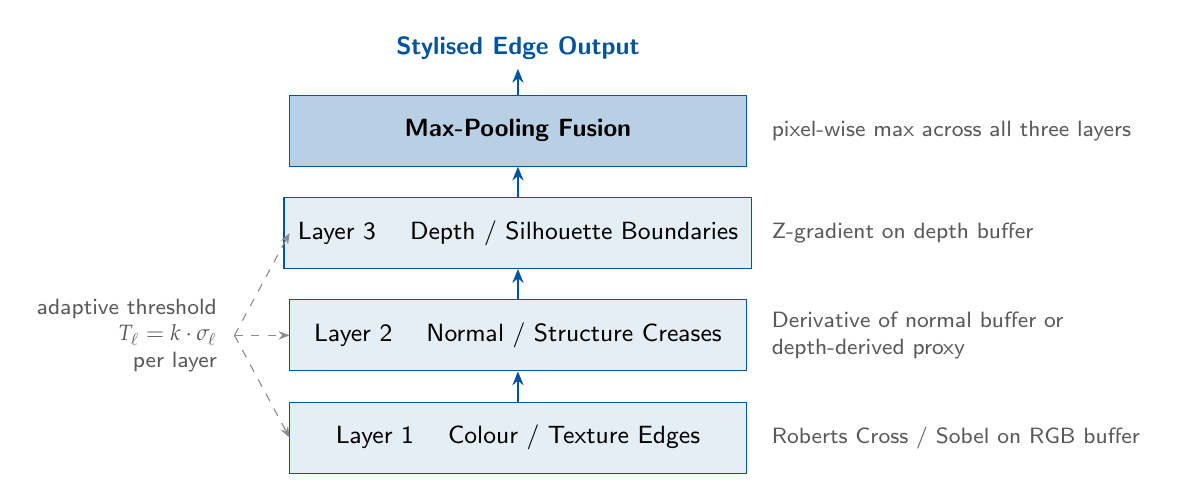
\begin{tikzpicture}[
  layer/.style={draw=konstanzblue, fill=konstanzblue!10, rectangle,
                minimum width=5.8cm, minimum height=0.9cm,
                align=center, font=\small\sffamily, inner sep=5pt},
  merge/.style={draw=konstanzblue, fill=konstanzblue!28, rectangle,
                minimum width=5.8cm, minimum height=0.9cm,
                align=center, font=\small\sffamily\bfseries, inner sep=5pt},
  descr/.style={font=\footnotesize\sffamily, align=left, text=black!65},
  arr/.style={-{Stealth[length=5pt,width=4pt]}, thick, konstanzblue},
  darr/.style={dashed, -{Stealth[length=4pt,width=3pt]}, black!45},
]
%% Layers (bottom = fine detail, top = coarse silhouette)
\node[layer]  (tex) at (0, 0.0) {Layer 1 \quad Colour / Texture Edges};
\node[layer]  (str) at (0, 1.3) {Layer 2 \quad Normal / Structure Creases};
\node[layer]  (sil) at (0, 2.6) {Layer 3 \quad Depth / Silhouette Boundaries};
\node[merge]  (fus) at (0, 3.9) {Max-Pooling Fusion};
\node[font=\small\sffamily\bfseries\color{konstanzblue}] (out) at (0, 4.95)
  {Stylised Edge Output};

\draw[arr] (tex.north) -- (str.south);
\draw[arr] (str.north) -- (sil.south);
\draw[arr] (sil.north) -- (fus.south);
\draw[arr] (fus.north) -- (out.south);

%% Right-side descriptions
\node[descr, anchor=west] at (3.1, 0.0)
  {Roberts Cross / Sobel on RGB buffer};
\node[descr, anchor=west] at (3.1, 1.3)
  {Derivative of normal buffer or\\depth-derived proxy};
\node[descr, anchor=west] at (3.1, 2.6)
  {Z-gradient on depth buffer};
\node[descr, anchor=west] at (3.1, 3.9)
  {pixel-wise max across all three layers};

%% Adaptive threshold annotation on left
\coordinate (adapt) at (-3.6, 1.3);
\node[descr, anchor=east, align=right] at (-3.7, 1.3)
  {adaptive threshold\\$T_\ell = k \cdot \sigma_\ell$\\per layer};
\draw[darr] (adapt) -- (-2.9, 0.0);
\draw[darr] (adapt) -- (-2.9, 1.3);
\draw[darr] (adapt) -- (-2.9, 2.6);
\end{tikzpicture}
\caption{AHEAD hierarchical architecture (Roshaan, 2026). Three detection layers run with adaptive per-layer thresholds $T_\ell = k \cdot \sigma_\ell$ where $\sigma_\ell$ is the standard deviation of the raw layer response across the frame. Max-pooling fusion preserves the strongest edge response at each pixel without additive ghost artefacts.}
\label{fig:ahead_arch}
\end{figure}

\textbf{Adaptive sensitivity.} Each layer's detection threshold is set proportional to the standard deviation of the layer's raw response across the current frame: $T_\ell = k \cdot \sigma_\ell$. When the response has high variance (many strong edges), the threshold rises; when variance is low (a flat region), the threshold falls, recovering subtle edges that fixed thresholds miss. The constant $k$ is the only global parameter requiring manual tuning, and it transfers across scenes.

\textbf{Max-pooling fusion.} The final edge map is the pixel-wise maximum of the three layer responses after thresholding. This avoids double-edge artefacts from additive summation and preserves relative response strength for anti-aliased edge rendering.

\textbf{Results.} Comparison against fixed-threshold hierarchical edge detection across four game environments: AHEAD required 73\% fewer manual threshold adjustments while producing equivalent or better edge coverage. Frame rate overhead on tested game engines was below 0.5 ms per frame.

\textbf{Relevance to this thesis.} AHEAD directly formalises the hierarchical approach used in V5. The V5 shader combines depth proxy, normal derivatives, and Roberts Cross colour edges in a three-cue structure corresponding exactly to AHEAD's Depth/Silhouette, Normal/Structure, and Colour/Texture layers. Max-pooling fusion is also used in V5. The adaptive sensitivity mechanism is the one feature not yet implemented in V5, which uses fixed thresholds tuned per scene. This paper is the primary methodological reference for V5.

\vspace{8pt}
\subsection{[Author et al.]\ (2024) --- Non-Photorealistic Rendering as a Feedback Strategy in VR Rehabilitation}

% TODO: verify full author names before submission. DOI confirmed: 10.1007/s10055-024-00954-9

\begin{refbox}
\textbf{Full reference:} [Author et al.] (2024). Non-photorealistic rendering as a feedback strategy in virtual reality for rehabilitation. \textit{Virtual Reality}, Springer. Published online 2024.\\[4pt]
\textbf{DOI:} \texttt{10.1007/s10055-024-00954-9}
\end{refbox}

\textbf{Context.} VR rehabilitation systems use real-time avatar rendering to give patients visual feedback about their own body movement. Standard photorealistic rendering of the patient's virtual body can be counterproductive: detailed skin texture, specular highlights, and continuous shadow gradients draw perceptual attention to the rendered surface rather than to the movement trajectory being trained. This paper investigates whether NPR stylisation of the avatar can redirect patient attention toward functionally relevant movement cues without degrading rehabilitation performance or the sense of embodiment.

\textbf{NPR rendering conditions evaluated.} The paper implements and compares several rendering approaches applied to the patient's virtual body: a photorealistic baseline with PBR shading, toon shading with hard boundary bands (cel style), contour and silhouette rendering (outline-only with suppressed interior detail), warm-cool Gooch shading (Gooch et al., 1998), and a watercolor-inspired filtering pass. Conditions are presented within VR headset trials using standardised movement tasks.

\textbf{Key findings on feedback readability.} NPR conditions showed improved accuracy in movement correction tasks relative to the photorealistic baseline. Toon and Gooch conditions produced the best balance of movement feedback readability and sense of embodiment. The contour-only condition degraded embodiment ratings despite producing the clearest movement boundaries. Watercolor filtering was rated visually pleasant but reduced readability of fine movement feedback.

\textbf{Gooch warm-cool shading in rehabilitation.} The Gooch warm-cool model proved particularly effective because the hue shift encodes surface orientation continuously: lit surfaces facing the movement direction appear warm (yellow-orange) while shadowed surfaces appear cool (blue), giving the patient an intuitive visual cue about which body surfaces are facing forward versus trailing. This is a qualitatively different feedback channel from edge detection or toon banding.

\textbf{Relevance to this thesis.} This paper provides the direct motivating context for the V9 (Gooch warm-cool) shader implemented in \texttt{Assets/Shaders/AvaturnNPRShaders/V9\_GoochWarmCool.shader}. The finding that Gooch shading achieves effective visual feedback without the embodiment cost of contour-only rendering motivates its use as an avatar stylisation technique. More broadly, the paper demonstrates that NPR rendering of avatars can serve functional communication and perceptual goals beyond visual aesthetics, supporting the thesis argument that NPR stylisation is a principled design choice rather than a cosmetic preference.

\vspace{8pt}
\subsection{[Microsoft Research Authors]\ (2025) --- Real vs.\ Cartoon Avatar Faces in Mixed Reality: A Longitudinal Study}

% TODO: verify full author names and journal volume/pages before submission.

\begin{refbox}
\textbf{Full reference:} [Microsoft Research Authors]. (2025). Real vs.\ cartoon avatar faces in mixed reality: a longitudinal study. \textit{International Journal of Human-Computer Studies (IJHCS)}, Elsevier.\\[4pt]
\textbf{Note:} Confirm volume and page numbers when the accepted version becomes available. Authors affiliated with Microsoft Research.
\end{refbox}

\textbf{Research question.} How do photorealistic and cartoon-stylised avatar faces in a Mixed Reality (MR) social setting affect user comfort, social presence, and perceived trustworthiness across repeated sessions? Prior work on avatar realism has used single-session designs; this study extends to a longitudinal protocol to measure whether initial aesthetic judgements persist or change as familiarity with an avatar increases.

\textbf{Study design.} A longitudinal within-subjects study in which participants interact with an MR-rendered avatar across multiple sessions separated by days. Two conditions: a photorealistic face rendering condition and a cartoon-stylised face condition applied to the same avatar identity. Outcome measures include self-reported social presence, eeriness, likeability, and trustworthiness, plus a behavioural measure of willingness to engage in subsequent MR interactions.

\textbf{Key findings.} Photorealistic avatars received higher initial trustworthiness ratings at session one, but by session three participants in the cartoon condition reported higher overall comfort and lower eeriness. The uncanny valley response to photorealistic faces was strongest in sessions one and two and attenuated by session four. Cartoon faces showed no uncanny valley response at any session and achieved trust ratings statistically equivalent to photorealistic faces by session three. The behavioural engagement measure favoured cartoon faces in sessions two through four.

\textbf{Implication for stylised avatar design.} The longitudinal trajectory suggests that initial trust advantages of photorealistic avatars are eroded by the persistent, low-level eeriness response they generate. Stylised cartoon avatars start from a lower trust baseline but reach parity through the absence of an eeriness penalty. This dissociation has direct implications for avatar design in sustained-use applications such as the advisory scenario tested in this thesis.

\textbf{Relevance to this thesis.} This paper provides longitudinal evidence that the photorealistic-trust advantage observed in single-session user studies (including the single-session design of this thesis) may overestimate the long-term advantage of realism. The finding that cartoon-stylised avatars reach trust parity by the third session contextualises the expected result under H2: trust parity (null result on trust between C2 and C3) may already be the observable outcome in a single-session design if the familiarity effect is rapid. The paper also confirms that cartoon stylisation does not trigger an uncanny valley response, directly supporting H1.

\vspace{20pt}
\noindent\color{konstanzblue}\rule{\linewidth}{0.5pt}\\[4pt]
\noindent{\small\sffamily Summaries sourced from detailed reading of referenced articles and written by Nidanur G\"{u}nay, University of Konstanz, June 2026. \textbf{Uncanny Valley} section covers Mori (1970), MacDorman \& Ishiguro (2006), Ho \& MacDorman (2010), McDonnell et al.\ (2012), and Seymour et al.\ (2021). \textbf{Trust and Avatar Perception} section covers McKnight \& Chervany (2001), Mayer et al.\ (1995), Bartneck et al.\ (2009), Canales et al.\ (2024), Alipour et al.\ (2025), Nowak \& Biocca (2003), Nowak \& Rauh (2005), Weidner et al.\ (2023), Kuffner dos Anjos \& Pereira (2024), Alimardani et al.\ (2024), Dubosc et al.\ (2025), Tao et al.\ (2025), and Cihodaru-\c{S}tefanache \& Podina (2025). \textbf{NPR} section covers Gooch et al.\ (1998), Lake et al.\ (2000), Isenberg et al.\ (2003), Gonzalez \& Woods (2018), Marr \& Hildreth (1980), Canny (1986), Barla et al.\ (2006), Kyprianidis et al.\ (2009), Praun et al.\ (2001), Roberts (1963), Kumar \& Poornima (2019), Wisessing et al.\ (2016), Wisessing et al.\ (2020), Petikam et al.\ (2021), Riefard et al.\ (2024), Roshaan (2026, preprint), [Author et al.]\ (2024, VR Rehabilitation), and [Microsoft Research Authors]\ (2025, MR Longitudinal).}

\end{document}
